\documentclass[11pt]{article}

\usepackage{amsthm}
\usepackage{amsmath}
\usepackage{amssymb}
\usepackage{amsfonts}
\usepackage{graphicx}
\usepackage{color}
\usepackage{enumerate}
\usepackage{amscd}

\usepackage{longtable}


\usepackage{algorithm}
\usepackage{algorithmicx}
\usepackage{algpseudocode}

\usepackage[sort&compress,numbers]{natbib}


\usepackage{newtxtext,newtxmath}

%\usepackage[scaled]{helvet}
%\renewcommand\familydefault{\sfdefault}
%\usepackage[T1]{fontenc}





\usepackage{tikz-cd}
\usepackage[hyphens]{url}
\usepackage{wrapfig}
\usepackage{mathrsfs}
\usepackage{mdframed}

\usepackage{dsfont} % blackboard numerals

\usepackage{geometry}
\geometry{margin=0.75in}

\usepackage{setspace}
\usepackage[colorlinks,linkcolor=black,citecolor=black,urlcolor=blue]{hyperref}

%\usepackage{endfloat}



\newcommand{\R}{\mathbb{R}}
\newcommand{\E}{\mathbb{E}}
\newcommand{\Econd}{\E_{\Yij|\Yinj,\xinj}}
\newcommand{\EXY}{\E_{\Yinj,\xinj}}
\newcommand{\Prob}{\mathbb{P}}
\newcommand{\LDGP}{L^{\text{DGP}}}
\newcommand{\lDGP}{l^{\text{DGP}}}
\newcommand{\lcox}{l^{\text{Cox}}}
\newcommand{\lpois}{l^{\text{Pois}}}
\newcommand{\hazt}{\lambda_{ij}(t)}
\newcommand{\Yij}{Y_{ij}}
\newcommand{\Yik}{Y_{ik}}
\newcommand{\Yinj}{Y_{i-j}(t)}


\newcommand{\cDE}{\text{\it cDE}}
\newcommand{\mDE}{\text{\it mDE}}
\newcommand{\mPE}{\text{\it mPE}}

\newcommand{\xij}{x_{ij}}
\newcommand{\xik}{x_{ik}}
\newcommand{\xinj}{x_{i-j}}
\newcommand{\tij}{t_{ij}}
\newcommand{\tik}{t_{ik}}
\newcommand{\T}{\mathbf{T}}
\newcommand{\V}{\mathbf{V}}
\newcommand{\W}{\mathbf{W}}
\newcommand{\X}{\mathbf{X}}
\newcommand{\Y}{\mathbf{Y}}
\newcommand{\Z}{\mathbf{Z}}
\newcommand{\bH}{\mathbf{H}}
\newcommand{\bL}{\mathbf{L}}
\newcommand{\h}{\mathbf{h}}
\newcommand{\x}{\mathbf{x}}
\newcommand{\y}{\mathbf{y}}
\newcommand{\z}{\mathbf{z}}
\newcommand{\w}{\mathbf{w}}

\newcommand{\bomega}{\boldsymbol{\omega}}
\newcommand{\bxi}{\boldsymbol{\xi}}
\newcommand{\btheta}{\boldsymbol{\theta}}
\newcommand{\bphi}{\boldsymbol{\phi}}
\newcommand{\balpha}{\boldsymbol{\alpha}}
\newcommand{\betapois}{\hat{\beta}_{\text{Pois}}}
\newcommand{\betacox}{\hat{\beta}_{\text{Cox}}}
\newcommand{\betaDGP}{\hat{\beta}_{\text{DGP}}}
\newcommand{\betaPA}{\hat{\beta}_{\text{PA}}}
\newcommand{\er}{\text{error}}
\newcommand{\omegastar}{\omega^{\textstyle{*}}}
\newcommand{\etastar}{\eta^{\textstyle{*}}}

\newcommand{\dx}[1]{\ \text{d} #1}
\newcommand{\indicator}[1]{\mathds{1}\!\left\{ #1 \right\}}
\newcommand{\indep}{\ \rotatebox[origin=c]{90}{$\models$}\ }
\newcommand{\nindep}{\not\!\perp\!\!\!\perp}

\newcommand{\comments}[1]{[\textcolor{red}{#1}]}
\newcommand{\ZLcomment}[1]{[\textcolor{red}{Richard: #1}]}
\newcommand{\red}[1]{\textcolor{red}{#1}}
\newcommand{\blue}[1]{\textcolor{blue}{#1}}

\newtheorem{thm}{Theorem}[section]
\newtheorem{prop}{Proposition}
\newtheorem{cor}{Corollary}
\newtheorem{lem}{Lemma}
\newtheorem{defn}{Definition}

\setlength{\bibsep}{0.0pt}
\setlength{\parskip}{1em}
\setlength{\parindent}{0.0pt}


\allowdisplaybreaks


% Blinding for peer review: set to 1
\newcommand{\blind}{0}


\title{A model for COVID-19 transmission in Connecticut}

\author{Olga Morozova$^{1}$,
  Zehang Richard Li$^1$,
and Forrest W. Crawford$^{1,2,3,4}$  \\[1em]
\small 1. Department of Biostatistics, Yale School of Public Health \\
\small 2. Department of Statistics \& Data Science, Yale University \\
\small 3. Department of Ecology \& Evolutionary Biology, Yale University \\
\small 4. Yale School of Management }



%%%%%%%%%%%%%%%%%%%%%%%%%%%%%%%%%%%%%%%%%%%%%%%%%%%%%%%%%

\begin{document}

\maketitle

%%%%%%%%%%%%%%%%%%%%%%%%%%%%%%%%%%%%%%%%%%%%%%%%%%%%%%%


%%%%%%%%%%%%%%%%%%%%55

\section{Introduction}


Epidemiological models of disease transmission play an important role in supporting public health decision-making. Trajectories from these models can provide insights into the historical trends in epidemic dynamics or future outcomes under hypothetical intervention scenarios. 
%, i.e. estimates of the $R_0$ (basic reproductive number) or $R\textsubscript{eff}$ (effective reproductive number) that accounts for the effects of interventions intended to slow down transmission and depletion of susceptible individuals.
Transmission models are especially useful in situations of high uncertainty, offering a structured way to assess the potential effects of interventions under hypothetical scenarios.  Models cannot predict the future with certainty, but they can be helpful for scenario analysis by bounding the range of plausible future trajectories under assumptions about transmission \citep{holmdahl2020wrong}. 

Most US states implemented social distancing measures and stay-at-home orders to slow transmission of SARS-CoV-2. 
%, which, if remained uncontrolled, would have likely quickly overwhelmed health care system leading to a large number of deaths. 
As many states, including Connecticut, begin phased lifting of stay-at-home orders, public officials and public health policymakers are faced with several questions: 1) How effective are public health interventions like social distancing and stay-at-home orders in reducing cases, hospitalizations, and deaths? 2)  How should public health interventions be implemented in the future to minimize the risk of a resurgence? 3) What will be the effect of phased reopening plans?  Mechanistic transmission models can help answer these questions. When models are developed with a primary goal to support decision-making, they must balance parsimony and realism. Projection models should be simple enough to provide clear outputs in a timely manner with assumptions that can be understood by policymakers. At the same time, for such models to be useful, they need to be flexible enough to accommodate various sets of scenarios and give projections of epidemiologic features that may be needed by different stakeholders. 

Many of the nation-wide COVID-19 forecasting models that have been developed in the United States either do not use local data, or make simplifying assumptions not appropriate for localities \citep{cdc2020covid19forecasts}. These models may capture the country-wide dynamics, but are less useful for supporting decision-making in individual states or counties. Several nation-wide models have been developed with a goal to provide projections at the state level, but they usually use the same set of assumptions and estimates of key model parameters across all states, and may or may not be able to capture important local variations. For example, the COVID Act Now project \citep{covidactnow2020you} estimates that between April 13 - May 15, 2020, a 100\% of ICU rooms have been occupied in Connecticut, and that if all restriction are lifted, over 70\% of population would be infected and over 19,000 deaths would occur in the state before August 14th, 2020. Under current level of restrictions, the projections predict 26\% of population being infected and a total of 5,000 deaths by the same date. These projections may offer a useful snapshot of two hypothetical scenarios, but do not provide enough flexibility to estimate potential epidemic dynamics under partial lifting of restrictions, improved testing, increased hospitalization capacity, or a different set of assumptions about highly uncertain parameters.  

In this technical report, we introduce a county-structured transmission model of SARS-CoV-2 transmission and COVID-19 disease progression in Connecticut.  The model was developed with a goal to support intervention planning and decision-making in Connecticut, but could be adapted to other states or regions.  This report provides an in-depth technical description of the model and data calibration approach, along with results in Connecticut.  Additional COVID-19 reports for Connecticut in this series are available from \url{https://crawford-lab.github.io/covid19_ct/}. 

%%%%%%%%%%%%%%%%%%

\section{Model specification}

We developed a deterministic compartmental model of SARS-CoV-2 transmission and COVID-19 disease progression.
The model is based on the SEIR (Susceptible, Exposed, Infectious, Recovered) framework \citep{keeling2011modeling}, which we extend to accommodate distinct features of COVID-19 disease. We calibrate the model to observed dynamics of deaths and hospitalizations in Connecticut, and produce estimates of incidence and prevalence that may be helpful in designing population-level surveys. Similar models have been published recently, offering intervention effect estimates and projections in various locations \citep{cdc2020covid19forecasts, li2020substantial, kissler2020projecting, childs2020impact, salje2020estimating, salomon2020defining}.

Figure \ref{fig:model} shows a schematic representation of the model structure. We categorize infections as asymptomatic, mild symptomatic, and severe. Only severe infections may lead to death. Severe infections are defined as those requiring hospitalization. Since one of the key observable features of the model is dynamics of hospitalizations in the community, we use separate compartments for community hospitalizations and for severe cases occurring in closed communities, such as nursing homes, assisted living facilities, or prisons. Case fatality ratio (CFR) among severe cases in closed communities is assumed to be higher than the community hospital CFR.  If hospitalization capacity is overwhelmed, some severe cases in the community are denied hospitalization, and experience a higher probability of death compared to hospitalized cases. Mild symptomatic infections are assumed to self-isolate shortly after they develop symptoms and remain isolated until they recover. During the infectiousness period of symptomatic cases, we assume a period of presymptomatic viral shedding, i.e. the latency period is shorter than incubation period \citep{furukawa2020evidence}. In line with other similar models, we assume that asymptomatic cases exert lower force of infection, but remain infectious for a longer period of time, since they are less likely to self-isolate in the absence of widespread testing \citep{childs2020impact, salomon2020defining}.  The average time that severe cases spend in the infectious state is approximated by the time between onset of infectiousness and hospitalization (or attempted hospitalization in case of hospital overflow). Since severe cases are likely to be isolated at home before hospitalization, and those in nursing homes, assisted living facilities, or prisons likely get isolated within a few days after symptom onset, we use an ``isolation coefficient'' to reduce the effective force of infection from severe infectious compartment to avoid using an extra transient isolation compartment. Force of infection from hospitalized patients to unhospitalized susceptible individuals is assumed to be negligible. We assume that recovered individuals remain immune to reinfection for the duration of modeling period.  The model is implemented at the level of individual counties in Connecticut assuming that most contacts are happening within a given county. A small proportion of contacts is allowed to happen between adjacent counties. 

\begin{figure}
	\begin{center}
		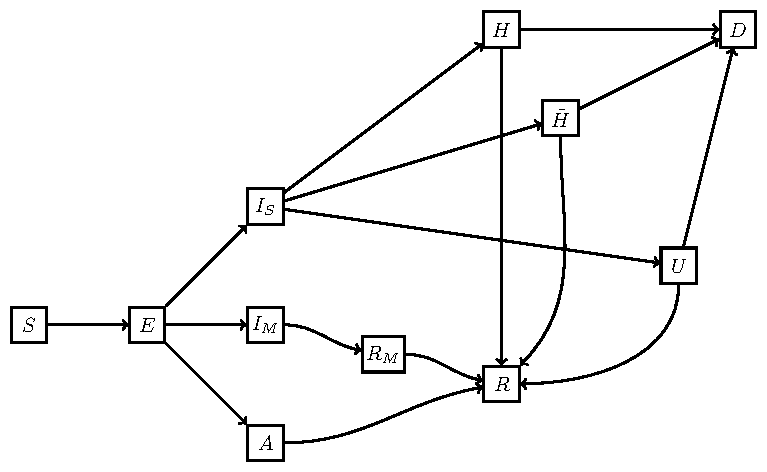
\includegraphics[width=0.65\textwidth]{model_diagram_ct.pdf}
	\end{center}
	\caption{Schematic illustration of the SARS-CoV-2 transmission model and COVID-19 disease progression structure.  Individuals begin in the susceptible ($S)$ compartment. Exposed individuals ($E$) may develop either asymptomatic ($A$), mild ($I_M$), or severe ($I_S$) infection. Asymptomatic and mild infections resolve without hospitalization and do not lead to death. Mild symptomatic cases self-isolate ($R_M$) shortly after development of symptoms, and transition to recovery ($R$) when infectiousness ceases. A proportion of severe cases require hospitalization ($H$) unless hospitalization capacity is exhausted, in which case they transition to $\bar{H}$ representing hospital overflow, then to recovery ($R$) or death ($D$). Some severe cases, including nursing homes and assisted living facilities residents, people in prisons, or individuals, who do not have access to hospitalization for other reasons, transition to compartment $U$ and may later recover or die. The model assumes a closed population without births and does not capture non-COVID-19 deaths.}
	\label{fig:model}
\end{figure}


%%%%%%%%%%%%%%%%%%%%%%%%%%%%%%%%%%%%%%%%%%%%%%%

\subsection{Compartmental model}

The model divides the population into 11 compartments: susceptible ($S$), exposed, latent infections ($E$), infectious and asymptomatic ($A$), infectious and mild symptomatic ($I_M$), infectious and severe ($I_S$), isolated mild infections removed from the pool of infectious individuals ($R_M$), hospitalized ($H$), severe in need of hospitalization, but denied it due to hospital capacity overflow ($\bar{H}$), severe in nursing homes, prisons or otherwise not having access to hospitalization ($U$), recovered ($R$), and died ($D$).  Transmission dynamics for county $i$  are given by the following system of ordinary differential equations: 
\[ \frac{\dx{S^{(i)}}}{\dx{t}} = -\beta S^{(i)} \left[ (1-k_n) \frac{ I_M^{(i)} + k_{I_S} I_S^{(i)} + k_A A^{(i)}}{N_i} + \frac{k_n}{|J_i|} \sum_{j\in J_i}  \frac{I_M^{(j)} + k_{I_S} I_S^{(j)} + k_A A^{(j)}}{N_j} \right], \]
where $N_i$ the population size of county $i$ and $J_i$ is the set of counties adjacent to county $i$.
\[ \frac{\dx{E^{(i)}}}{\dx{t}} = \beta S^{(i)} \left[ (1-k_n) \frac{ I_M^{(i)} + k_{I_S} I_S^{(i)} + k_A A^{(i)}}{N_i} + \frac{k_n}{|J_i|} \sum_{j\in J_i}  \frac{I_M^{(j)} + k_{I_S} I_S^{(j)} + k_A A^{(j)}}{N_j} \right] - \delta E^{(i)} \]
\[ \frac{\dx{A^{(i)}}}{\dx{t}} = q_A \delta E^{(i)} - \alpha_A A^{(i)} \]
\[ \frac{\dx{I_M^{(i)}}}{\dx{t}} = q_{I_M} \delta E^{(i)} - \alpha_{I_M} I_M^{(i)} \]
\[ \frac{\dx{R_M^{(i)}}}{\dx{t}} = \alpha_{I_M} I_M^{(i)} - \gamma_{R_M} R_M^{(i)} \]
\[ \frac{\dx{I_S^{(i)}}}{\dx{t}} = q_{I_S} \delta E^{(i)} - \alpha_{I_S} I_S^{(i)} \]
\[ \frac{\dx{H^{(i)}}}{\dx{t}} =  q_H (1 - \rho^{(i)}) \alpha_{I_S} I_S^{(i)} - \gamma_H H^{(i)}  \]
\[ \frac{\dx{\bar{H}^{(i)}}}{\dx{t}} =  q_H \rho^{(i)} \alpha_{I_S} I_S^{(i)} - \gamma_{\bar{H}} \bar{H}^{(i)},  \]
where $\rho^{(i)} = \left[ 1+\exp(0.5(C^{(i)}-H^{(i)})) \right]^{-1}$ is a ``soft'' hospitalization capacity overflow function, and $C^{(i)}$ represents hospitalization capacity in county $i$ at a given time point.
\[ \frac{\dx{U^{(i)}}}{\dx{t}} =  (1 - q_H) \alpha_{I_S} I_S^{(i)} - \gamma_{U} U^{(i)}  \]
\[ \frac{\dx{D^{(i)}}}{\dx{t}} = \gamma_H m_H H^{(i)} + \gamma_{\bar{H}}  m_{\bar{H}} \bar{H}^{(i)} + \gamma_{U} m_{U} U^{(i)} \]
\[ \frac{\dx{R}}{\dx{t}} = \alpha_A A^{(i)} + \gamma_{R_M} R_M^{(i)} + \gamma_H (1-m_H) H^{(i)} + \gamma_{\bar{H}} (1 - m_{\bar{H}}) \bar{H}^{(i)} + \gamma_{U} (1- m_{U}) U^{(i)}  \]



%%%%%%%%%%%%%%%%%%%%%%%%%%%%%%%%%%%%%%%%%%%%%%%

\subsection{Parameter definitions}

Table \ref{table:params} provides a list of model parameters and their definitions. Some of the parameters from Table \ref{table:params} are not directly used in the ODE system, but are used as inputs to compute other model parameters. \\ 
\comments{Add the rest of parameters here, including intervention effects}
\comments{I recommend you make this a regular table environment, single spacing, and let it float on the page}

%\begin{spacing}{0.9}
\begin{longtable} {p{.11\textwidth} p{.85\textwidth} }
	\caption{Model parameters } \\
	Notation & Definition \\[0.5em] \hline
	{} & {} \\
	\endfirsthead
	Notation & Definition  \\[0.5em] \hline
	\endhead
	{} & {}  \\[-1em]
	$\beta$ & Transmission parameter per $S-I$ pair \\[0.5em]
	$\delta$ & (Latency period)$^{-1}$ (days$^{-1}$) \\[0.5em]
	$q_A$, $q_{I_M}$, $q_{I_S}$  & Proportions of asymptomatic, mild symptomatic, and severe infections \\[0.5em]
	$q_H$ & Proportion of severe cases that will result in hospitalization or attempted hospitalization under hospital overflow \\ [0.5em]
	$q_{HD}$ & Proportion of all COVID-19 related deaths that occur in hospitals \\ [0.5em]
	$\alpha_A$ & (Duration of infectiousness among asymptomatic infections)$^{-1}$ (days$^{-1}$) \\[0.5em]	
	$\alpha_{I_M}$ & (Duration of infectiousness among mild symptomatic infections, time until isolation)$^{-1}$ (days$^{-1}$) \\[0.5em]
	$\gamma_{R_M}$ & (Duration of isolation among mild symptomatic infections, time to recovery)	$^{-1}$ (days$^{-1}$) \\[0.5em]
	$\alpha_{I_S}$ & (Duration of infectiousness among severe cases, time until hospitalization)$^{-1}$ (days$^{-1}$) \\[0.5em]	
	$\gamma_{H}$ & (Length of hospitalization, time until recovery or death)$^{-1}$ (days$^{-1}$) \\[0.5em]
	$\gamma_{\bar{H}}$ & (Remaining time until recovery or death among hospital overflow patients)$^{-1}$ (days$^{-1}$) \\[0.5em]
	$\gamma_{U}$ & (Remaining time until recovery or death among nursing home residents and alike)$^{-1}$ (days$^{-1}$) \\[0.5em]
	$k_A$ & Relative infectiousness of asymptomatic cases compared to symptomatic \\[0.5em]
	$k_{I_S}$ & Isolation coefficient among severe cases in nursing homes and those expecting hospitalization \\[0.5em]
	$m_H$ & Case fatality ratio among hospitalized severe cases \\[0.5em]
	$m_{\bar{H}}$ & Case fatality ratio among severe cases denied hospitalization due to hospital capacity overflow \\[0.5em]
	$m_{U}$ & Case fatality ratio among severe cases in nursing homes, prisons, or with no access to hospitalization \\[0.5em]
	$k_n$ & Proportion of all contacts that happen with individuals from adjacent counties (as opposed to within county) \\[0.5em]
	$C(t)$ & Hospitalization capacity at time $t$, may be constant or vary over time representing capacity increase intervention \\[0.5em]
	$w\textsubscript{school}$ & Maximum size of school closure effect on contact rate reduction \\[0.5em]
	$w\textsubscript{lockdown}$ & Maximum size of lockdown effect on contact rate reduction \\[0.5em]
	$w\textsubscript{testing, $A$}$ & Effect size of increased testing and contact tracing on the rate of removal (isolation) of asymptomatic infections \\[0.5em]
	$w\textsubscript{testing, $I_M$}$ & Effect size of increased testing and contact tracing on the rate of isolation of mildly symptomatic infections \\[0.5em]
	$L_H$, $L_D$ & Reporting lags of hospitalizations and deaths (days) \\[0.5em]
	$L_0$ & Lag of epidemic onset date, days before 03-01-2020 \\[0.5em]
	\hline
	\label{table:params}
\end{longtable}
%\end{spacing}


%%%%%%%%%%%%%%%%%%%%%%%%%%%%%%%%%%%%%%%%%5

\subsection{Geographic structure}

%\comments{Describe the contact structure for counties}
%\comments{Richard, could you generate a map of Connecticut with counties labeled, alongside a labeled adjacency matrix for counties? }
Figure \ref{fig:map} shows the county map of Connecticut along with the county adjacency matrix. The geographic boundary files were obtained from the Connecticut Department of Environmental Protection~\citep{shapefile}. We assume that a fraction $(1-k_n)$ of all contacts happen within a given county, and the remaining $k_n$ contacts happen between individuals residing in adjacent counties.

\begin{figure} %[htb]
	\centering
	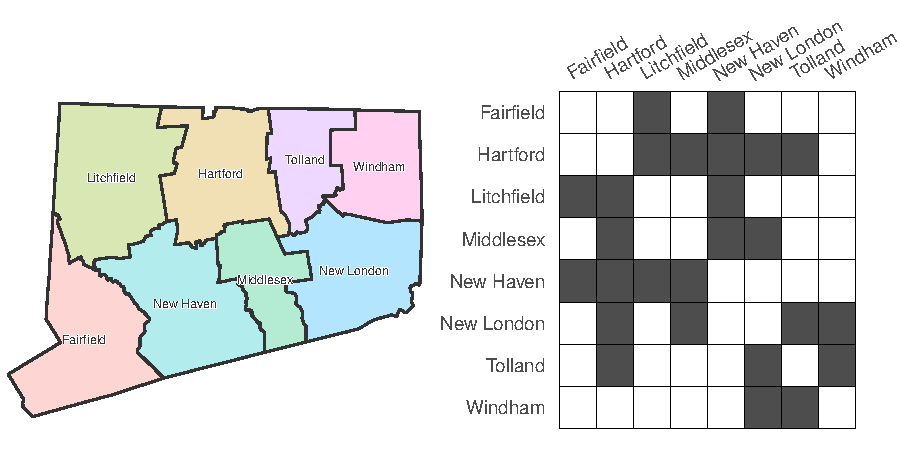
\includegraphics[width=.7\textwidth]{figures/map_adj.pdf}
	\caption{County map of Connecticut and county adjacency matrix.}
	\label{fig:map}
\end{figure}


%%%%%%%%%%%%%%%%%%%%%%%%%%%%%%%%%%%%%%%%%%%


\subsection{Effects of social distancing and testing interventions} 

Social distancing measures, in particular school closure and lockdown, reduce the value of transmission parameter $\beta$. The value of the transmission parameter at time $t$ is calculated as:
\[ \beta(t) = \beta_0 (1 - \iota\textsubscript{school}(t) ) (1 - \iota\textsubscript{lockdown} (t) ), \]
where $\beta_0$ is a value of transmission parameters in the absence of any interventions, $\iota\textsubscript{school}(t)$ is the proportion of contact reduction following school closure, and $\iota\textsubscript{lockdown} (t)$ is a proportion of contact reduction following lockdown that is independent of school closure effect. $\iota\textsubscript{school}(t)$ and $\iota\textsubscript{lockdown} (t)$ are zero when these interventions are not in effect, and can either have a constant or time-varying values when interventions are in effect. 

Based on the known dates of school closure and lockdown orders, and assuming that these effects are constant over time once they reach their maximum levels $w\textsubscript{school}$ and $w\textsubscript{lockdown}$, we calibrate the values of these effects to observed data. To project epidemic dynamics into the future, we replace  $\iota\textsubscript{lockdown} (t)$ with a step function representing post-lockdown increases in population-level contact.  Figures \ref{fig:slow_low} to \ref{fig:fast_high} show examples of assumed post-lockdown increases in contact, starting on May 20. 


Increase in testing capacity and contact-tracing is assumed to result in earlier identification and isolation of mild symptomatic and asymptomatic cases, and leads to increases in $\alpha_A$ (rate of transition from $A$ to $R$) and $\alpha_{I_M}$ (rate of transition from $I_M$ to $R_M$). The values of the transition rates at time $t$ are calculated as:

\[ \alpha_A(t) = \alpha_A^{(0)} (1 + \iota\textsubscript{testing, $A$} (t)) \]
\[ \alpha_{I_M}(t) = \alpha_{I_M}^{(0)} (1 + \iota\textsubscript{testing, $I_M$} (t)), \]
where $\alpha_A^{(0)}$ and $\alpha_{I_M}^{(0)}$ are reciprocals of the duration of time until isolation among asymptomatic and mildly symptomatic infections respectively under current testing availability conditions. Similarly to the parametrization of distancing effects, $\iota\textsubscript{testing, $A$} (t)$ and $\iota\textsubscript{testing, $I_M$} (t)$ may vary over time. 
We assume that soon after the lockdown is lifted, testing capacity increases and remains constant at that level. The values of $\iota\textsubscript{testing, $A$} (t)$ and $\iota\textsubscript{testing, $I_M$} (t)$ are assumed to be zero prior to May 20, 2020 and increase to $w\textsubscript{testing, $A$}$ and $w\textsubscript{testing, $I_M$}$ respectively afterwards.  



%%%%%%%%%%%%%%%%%%%%%%%%%%%%%%%%%%%%%%%%%%%


\section{Model calibration and Bayesian posterior inference}


We estimate a joint posterior distribution of model parameters using the the observed dynamics of community hospitalizations and cumulative number of deaths.  Due to changing testing patterns and varying case ascertainment proportions over time, we do not use reported case counts in the calibration procedure.  The parameters in the transmission model are not simultaneously identifiable given the observed data. In particular, different sets of parameters that collectively determine early epidemic growth rate (i.e. transmission parameter $\beta$ and parameters that define force of infection) are observationally equivalent. Given this limitation, we fix a subset of parameters at their point estimates and estimate the remaining parameters using Bayesian posterior sampling.  To generate 95\% uncertainty intervals for projections, we sample from the joint posterior over estimated parameters and uncertainty distributions for fixed parameters. 

Several model parameters influence epidemic dynamics in the future, beyond the data available for calibration. These parameters include the case fatality ratio in the case of hospital overflow ($m_{\bar{H}}$), testing capacity and contact tracing effects ($w\textsubscript{testing, $A$}$ and $w\textsubscript{testing, $I_M$}$), and the extent of release of suppressed contact once lockdown is lifted. These parameters cannot be estimated based on historical data, but may be estimated in the future. For the purpose of projections, we impose a distribution on these parameters independent of one another and of the joint posterior distribution of calibrated parameters.  The point estimates of models parameters, prior distributions, and assumed distributions are summarized in Table \ref{table:priors}.


\subsection{Continuous transmission model parameters} 

Let $\btheta$ denote the subset of continuous transmission model parameters whose joint distribution is calibrated to observed data. For each individual parameter $\theta$, we specify a fixed support $[\theta\textsubscript{min}, \theta\textsubscript{max}]$, and put independent beta priors on the transformed parameter, i.e.,
\begin{equation}
\frac{\theta - \theta\textsubscript{min}}{\theta\textsubscript{max} - \theta\textsubscript{min}} \sim \mbox{Beta}(a_{\theta}, b_{\theta}),
\label{eq:truncdist}
\end{equation}    
where the shape parameters $a_{\theta}$ and $b_\theta$ are set to let $\theta$ have mean $\mu_\theta$ and standard deviation $\sigma_\theta$. Table \ref{table:priors} provides the list of $(\mu_\theta, \sigma_\theta, \theta\textsubscript{min}, \theta\textsubscript{max})$ for all parameters in $\btheta$. 


\subsection{Initial conditions}

Given a set of transmission parameters, we initialize the compartmental model by specifying the size of exposed ($E$) compartment in each county and setting the size of downstream compartments to be zero. The initial size of susceptible compartment is the population of a given county minus the size of exposed compartment. The initial size of exposed compartment in each county was set based on the relative population size and the dates of first registered case and deaths in that county. 
%These values are not required to be integers. 
We allow the date of epidemic onset to vary by setting the described initial conditions to correspond to day $-L_0$, where day $0$ corresponds to a calendar date of March 1, 2020. 
% The value of $L_0$ was calibrated to data as part of the MCMC algorithm. At each step of the algorithm, a proposed value of $L_0$ was sampled independently from a set of candidate values, i.e. $L_{0} \sim \mbox{Unif} \{l\textsubscript{min}, \ldots, l\textsubscript{max}\}$. 
The state of the system at any given time is therefore a deterministic function of the initial size of exposed compartment, model parameters, and $L_0$ that determines the date of epidemic onset. We put a uniform prior on $L_{0}$ over $\{l\textsubscript{min}, \ldots, l\textsubscript{max}\}$.



\subsection{Reported hospitalizations and deaths} 

We accommodate reporting lags in observed hospitalizations and deaths. Reporting lags are correlated with other unknown parameters, including latency period, epidemic onset lag, time between infection and hospitalization, time between infection and death, length of hospital stay, and difference in death reporting lags between hospitals and nursing homes. We model the observed hospitalizations $h(t)$ and deaths $d(t)$, given parameters $\btheta$, at time $t$ using a Poisson model,  
\begin{align}
h(t) &\sim \mbox{Poisson}(H(t, L_H, \btheta)), \\
d(t) &\sim \mbox{Poisson}(D(t, L_D, \btheta)), 
\end{align}
where $H(t, L_H, \btheta)$ and $D(t, L_D, \btheta)$ are model-projected current hospitalizations and cumulative deaths at time $t$ with reporting lags $L_H$ and $L_D$ under parameter values $\btheta$. We put uniform priors on $L_H$ and $L_D$ over a range of plausible values. 

% \comments{
% The hospitalizations and deaths data likelihood functions take a form:
% \begin{align}
% \mathcal{L}_{hosp. data} (\btheta | h(t_{h_1},\cdots, t_{h_K}) ) =  \prod_{t=t_{h_1}}^{t_{h_K}} \left[ f_{Pois} (h(t) | H(t, L_H , \btheta) ) \right]^{\frac{1}{K}} \\
% \mathcal{L}_{death. data} (\btheta | d(t_{d_1},\cdots, t_{d_M}) ) =  \prod_{t=t_{d_1}}^{t_{d_K}} \left[ f_{Pois} (d(t) | D(t, L_D , \btheta) ) \right]^{\frac{1}{M}}, 
% \end{align}
% where $f_{Pois}(x | \lambda) $ is a probability mass function of Poisson distribution with rate parameter $\lambda$, $K$ is number of observations in hospitalization data series, and $M$ is number of observations in death data series. The joint data likelihood function combines hospitalizations and deaths likelihoods:
% \begin{equation}
% \mathcal{L}_{data} (\btheta | h(t_{h_1},\cdots, t_{h_K}), d(t_{d_1},\cdots, t_{d_M}) ) =  \mathcal{L}_{hosp. data} (\btheta | h(t_{h_1},\cdots, t_{h_K}) ) \mathcal{L}_{death. data} (\btheta | d(t_{d_1},\cdots, t_{d_M}) )
% \end{equation}
% }

% \comments{
% Joint posterior distribution of $\btheta$ up to a normalizing constant is given by
% \begin{equation}
% f_{posterior}(\btheta) = \mathcal{L}_{prior} (\btheta | (\mu_{\btheta}, \sigma_{\btheta}, \btheta\textsubscript{min}, \btheta\textsubscript{max}) ) \mathcal{L}_{data} (\btheta | h(t_{h_1},\cdots, t_{h_K}), d(t_{d_1},\cdots, t_{d_M}) )
% \label{eq:posterior}
% \end{equation}
% }

The model above yields the following posterior distribution,
\begin{equation}
p(\btheta, \bL | h(t), d(t)) \propto p(\btheta) p(\bL)
							 \prod_t p\big(h(t)| H(t, L_H, \btheta)\big)
							         p\big(d(t)| D(t, L_D, \btheta)\big).
\label{eq:posterior}
\end{equation}
Sampling from the joint posterior distribution of $\btheta$ given in (\ref{eq:posterior}) is performed using Markov Chain Monte Carlo (MCMC). We implemented a Metropolis algorithm with symmetric Gaussian proposals for $\btheta$ and independent proposals for $\bL$. We ran the sampler for $200,000$ iterations and thinned the chain using every $5$-th iteration.


%%%%%%%%%%%%%%%%%%


\subsection{Parameter values, prior distributions, and data sources}

Asymptomatic infections play an important role in transmission of SARS-CoV-2 \citep{furukawa2020evidence}, but estimates of the proportion of infections that do not exhibit symptoms vary \citep{he2020estimation, nishiura2020estimation, mizumoto2020estimating, emery2020contribution}. The true proportion of asymptomatic infections is important for projections and policy planning due to its relationship to herd immunity. In the absence of reliable estimates of cumulative incidence based on sero-prevalence surveys, we consider three scenarios: 

\begin{enumerate}
	\item Scenario 1, low asymptomatic: $q_A = 0.36$
	\item Scenario 2, medium asymptomatic: $q_A = 0.5$
	\item Scenario 3, high asymptomatic: $q_A = 0.7$
\end{enumerate}

The value $q_A = 0.36$ was calculated as an age-adjusted weighted average of several estimates available in the literature.  
\citet{nishiura2020estimation} estimated 30.8\% among Japanese citizens evacuated from Wuhan, China and applied to age group 20-64 years old.  
\citet{mizumoto2020estimating} estimated 17.9\% among infections on the Diamond Princess cruise ship and applied to age group 65 plus years old
and we assumed 60\% for age group 0-19 years old, consistent with findings reported by \citet{russell2020estimating}, where 4 out of 6 infections in this age group were asymptomatic among passengers of the Diamond Princess. 
The average was weighted by the age distribution of Connecticut population. 
Based on recent evidence suggesting that the proportion of asymptomatic infections may be higher \citep{he2020estimation, emery2020contribution, kimball2020asymptomatic}, we assumed $q_A = 0.5$ and $q_A = 0.7$ in medium and high scenarios respectively.  

Table \ref{table:priors} provides a list of prior mean, standard deviation, and lower and upper bounds of the model parameters along with data sources. For parameters whose values were fixed, only the mean is given. In the three scenarios considered, we fixed the values of asymptomatic proportions ($q_A$). The proportion of severe cases ($q_{I_S}$) was allowed to vary with a mean assumed to be 10\% of symptomatic infections in line with \citep{verity2020estimates, bi2020epidemiology, salje2020estimating}. $q_{I_M}$ is calculated as $1 - q_A - q_{I_S}$. 

Duration of the latency period ($1/\delta$) was fixed, since reliable estimates of this parameter are available and because it is correlated with parameters that were allowed to vary, including reporting lags and parameters that determine duration of infectiousness and time between infection and recovery or death. We assume an average of 4 days of latency \citep{li2020substantial, salje2020estimating} and 1.5 days of presymptomatic infectiousness \citep{wei2020presymptomatic} resulting in an average incubation period of 5.5 days in line with \citep{lauer2020incubation, bi2020epidemiology, li2020early, linton2020incubation, he2020estimation, salje2020estimating}. 

A subset of parameters ($\alpha_A$, $k_A$, $\alpha_{I_M}$, $\alpha_{I_S}$, $k_{I_S}$) collectively determine force of infection at a given time. Force of infection and transmission parameter $\beta$ together
% , which combines contact frequency and transmission probability per contact, 
determine the early growth of the epidemic. Without additional data, these parameters cannot be simultaneously identified. We therefore fixed parameters for which estimates are available or can be calculated from available estimates ($\alpha_A$, $\alpha_{I_M}$, $\alpha_{I_S}$), and calibrate those that are unavailable ($k_A$, $k_{I_S}$). We assume a diffuse prior on $\beta$, which absorbs additional variations of parameters that determine force of infection. 

\begin{spacing}{.9}
	\begin{longtable}[H] {p{.15\textwidth} p{.07\textwidth} p{.07\textwidth} p{.07\textwidth} p{.07\textwidth} p{.38\textwidth} }
		\caption{Prior distributions of model parameters} \\
		Parameter & Mean & SD & Lower & Upper & Source   \\[0.5em] \hline
		{} & {} & {} & {} & {} & {} \\
		\endfirsthead
		Parameter & Mean & SD & Lower & Upper & Source  \\[0.5em] \hline
		{} & {} & {} & {} & {} & {}  \\
		\endhead
		$q_A$: low & 0.36 & {-} & {-} & {-} & \citep{nishiura2020estimation, mizumoto2020estimating, russell2020estimating}  \\[0.5em]
		$q_A$: medium & 0.5 & {-} & {-} & {-} & Assumed, in line with \citep{he2020estimation, emery2020contribution, kimball2020asymptomatic} \\[0.5em]
		$q_A$: high & 0.7  & {-} & {-} & {-} & Assumed, in line with \citep{he2020estimation, emery2020contribution, kimball2020asymptomatic} \\[0.5em]
		$q_{I_S}$ (low $q_A$) & 0.064 & 0.012 & 0.024 & 0.104 & 10\% of symptomatic infections \citep{verity2020estimates, bi2020epidemiology, salje2020estimating} \\[0.5em]
		$q_{I_S}$ (medium $q_A$) & 0.05 & 0.012 & 0.015 & 0.085 & 10\% of symptomatic infections \citep{verity2020estimates, bi2020epidemiology, salje2020estimating} \\[0.5em]
		$q_{I_S}$ (high $q_A$) & 0.03 & 0.0075 & 0.01 & 0.05 & 10\% of symptomatic infections \citep{verity2020estimates, bi2020epidemiology, salje2020estimating} \\[0.5em]
		$\beta$ (low $q_A$) & 1.25 & 0.5 & 0.25 & 2.25 & A diffuse prior assumed \\[0.5em]
		$\beta$ (medium $q_A$) & 1.5 & 0.5 & 0.25 & 2.75 & A diffuse prior assumed \\[0.5em]
		$\beta$ (high $q_A$) & 2 & 0.5 & 0.75 & 2.75 & A diffuse prior assumed \\[0.5em]
		$\delta$ & 1/4 & {-} & {-} & {-} & \citep{lauer2020incubation, bi2020epidemiology, li2020early, linton2020incubation, he2020estimation, salje2020estimating, wei2020presymptomatic} \\[0.5em]
		$\alpha_A$ & 1/7 & {-} & {-} & {-} & \citep{wolfel2020virological} \\[0.5em]
		$\alpha_{I_M}$ & 1/4 & {-} & {-} & {-} & \citep{salje2020estimating, li2020substantial, kissler2020projecting}; of 4 days, 1.5 is assumed to be presymptomatic \citep{wei2020presymptomatic} \\[0.5em]
		$\gamma_{R_M}$ & 1/7 & {-} & {-} & {-} & \citep{wolfel2020virological, cdc2020isolation} \\[0.5em]
		$\alpha_{I_S}$ & 1/9.5 & {-} & {-} & {-} & \citep{verity2020estimates, lewnard2020incidence} \\[0.5em]
		$\gamma_H$, $\gamma_{\bar{H}}$ & 1/10 & 0.015 & 0.06 & 0.14 & \citep{lewnard2020incidence, paranjpe2020clinical}, data from Yale Hew Haven Hospital \\[0.5em]
		$\gamma_U$ & 1/14 & 0.01 & 0.03 & 0.11 & Assumed \\[0.5em]
		$k_A$ & 0.4 & 0.05 & 0.25 & 0.55 & \citep{salomon2020defining, ferguson2020impact} \\[0.5em]
		$k_{I_S}$ &  0.7 & 0.05 & 0.55 & 0.85 & Assumed \\[0.5em]
		$m_H$ & 0.2 & 0.015 & 0.155 & 0.245 & \citep{lewnard2020incidence, paranjpe2020clinical, petrilli2020factors, verity2020estimates, CHAwebsite} \\[0.5em]
		$m_U / m_H$ & 1.5 & 0.15 & 1.1 & 1.9 & Assumed \\[0.5em]
		$m_{\bar{H}} / m_H$ & 1.5 & 0.25 & 1 & 2 & Assumed \\[0.5em]
		$q_{HD}$ & 0.48 & 0.01 & 0.43 & 0.53 & \citep{CHAwebsite, DPHwebsite} \\[0.5em]		
		$q_H$ & 0.58 & {-} & {-} & {-} & {Calculated based $q_{HD}$ and $m_U/m_H$} \\[0.5em]
		$k_n$ & 0.015 & {-} & {-} & {-} & Assumed \\[0.5em]
		\hline
	\label{table:priors}
	\end{longtable}
\end{spacing}

% $q_{HD}$ denotes proportion of all COVID-19 related deaths that occur in hospitals.

\textbf{Initial conditions and reporting lags}\\[0.5em]
Based on the relative population size of the counties and the date of first registered case and death, we assume an initial size of exposed compartment to be 7.5 in Fairfield, 6.5 in Hartford, 0 in Litchfield, 0.25 in Middlesex, 4.5 in New Haven, 0.13 in New London, 0.05 in Tolland and 0.04 in Windham. We allow the starting date of the epidemic to be between February 14th - 20th and calibrate a scenario-specific distribution of starting dates to the observed data. 

Early in the epidemic, many infections were likely imported from New York City, which experienced a major outbreak in the spring of 2020. In particular, many residents of Fairfield county work in New York City. We do not directly model importation events, and the pre-specified number of exposed individuals in Fairfield does not include all infection importation events, which likely happened in the course of several days or even weeks. This unaccounted force of infection early in the epidemic got absorbed in the estimation of transmission parameter $\beta$.

We specified a wide range of reporting lags for hospitalizations and deaths, resulting in ranges of 4-7 days for hospitalizations and 7-11 days for deaths. It is likely that deaths occurring in hospitals are reported with substantially smaller lag than those occurring in nursing homes, since many of them need to be confirmed by a medical examiner.  

\textbf{Reduction in transmission following school closure and lockdown orders} \\[0.5em]
We calibrated the parameters that determine reduction in contact rates following school closure and lockdown orders to the observed data. 
We assume that $\iota\textsubscript{school}(t)$ equals zero before March 13th, 2020 - the date of school closure order, and equals some constant positive value $w\textsubscript{school}$ afterwards. 
The  $\iota\textsubscript{lockdown} (t)$ equals zero before March 20th, 2020 - the date of lockdown order, and equals some positive values $w\textsubscript{lockdown}$ after March 22nd, 2020 - the date when the lockdown order took effect. Between March 20th - March 22nd, 2020 the value of $\iota\textsubscript{lockdown} (t)$ is smoothly increasing from zero to $w\textsubscript{lockdown}$. 
Since the dates of school closure and lockdown orders are very close, it is difficult to simultaneously identify $w\textsubscript{school}$ and $w\textsubscript{lockdown}$. We therefore put a narrow prior distribution on $w\textsubscript{school}$ and wide on $w\textsubscript{lockdown}$ with a restriction $ 0 < (w\textsubscript{school} + w\textsubscript{lockdown}) < 1$ . 


\textbf{Observed data} \\[0.5em]
% Cumulative deaths were obtained from the New York Times coronavirus data repository~\citep{nyt2020Connecticut}. 
Cumulative deaths and current hospitalizations were obtained from Connecticut Department of Public Health daily reports~\citep{DPHwebsite} and the Connecticut Hospital Association~\citep{CHAwebsite}. 
We calculated county-level population and age structure in Connecticut using the 2014--2018 estimates of the American Community Survey~\citep{acs2018}. 
Daily total available hospital beds (including occupied) in each county were obtained from the Connecticut Hospital Association~\citep{CHAwebsite} and used as hospitalization capacity values on a given date. The latest available value of hospitalization capacity was used for future projections.

% We used data from the United States Census Bureau to estimate county-level population and age structure in Connecticut \citep{bureau2020american} \comments{give the correct reference}. 
% \comments{Richard, can  you please describe hospitalization capacity estimation}

%Parameter estimates are obtained considering \citet{zhao2020mathematical, russell2020estimating, riou2020adjusted, riou2020pattern, prem2017projecting, nishiura2020estimation, mossong2008social, liu2020contribution, linton2020incubation, li2020substantial, li2020early, funk2018socialmixr}.
%Detailed description of model parameters and equations is provided in the Appendix. \ZLcomment{Not sure if we want to write more explicitly some of the parameters (probably fixed ones)? Something like: ``We assumed an incubation period of X days[ref]''?}


% We estimated county-level population age distributions using American Community Survey 2013-2017 5-year Data Release \citep{bureau2020american}. We used Florida's hospital bed counts reported by \citet{chen2020florida}, which was based on Medicare cost reports for fiscal year 2017. Then, we aggregated bed counts for each county. Cases, hospitalizations and deaths counts were obtained longitudinally from \citet{noauthor2020covid19}.

%Age related: Age-specific transmissibility \citep{zhao2020mathematical}; age-adjusted data from the outbreak on the diamond princess cruise ship \citep{russell2020estimating}; case fatality ratio in Wuhan \citep{riou2020adjusted}.
%Pattern of early human-to-human transmission \citep{linton2020incubation}.
%social contact matrices \citep{prem2017projecting}.
%ratio of novel coronavirus infections \citep{nishiura2020estimation}.
%Social contacts and mixing patterns \citep{mossong2008social}.
%contribution of pre-symptomatic transmission \citep{liu2020contribution}.
%Incubation period \citep{linton2020incubation}.
%undocumented infection \citep{li2020substantial}.
%Early transmission dynamics  \citep{li2020early}.

%%%%%%%%%%%%%%%%%%%%%%%%%%%%%%%%%%%%%%%%%%%%%%%5



\section{Results}


Figure \ref{fig:fit} shows calibrated projections of hospitalizations and deaths, with 95\% uncertainty intervals, under the low asymptomatic fraction scenario and observed data as dots.  Observed data points track with mean projections and largely fall within uncertainty intervals.  Calibration results under medium and high asymptomatic fraction scenarios demonstrate a similar fit to historical data.  
Table \ref{tbl:posterior} reports means and 95\% credible intervals of marginal posterior distributions of model parameters under the three asymptomatic fraction scenarios.

Figures \ref{fig:slow_low} to \ref{fig:slow_high} summarize projections under the low, medium and high asymptomatic fraction and `slow' reopening. Slow reopening assumes that at one-month intervals, 10\% of the suppressed contact (relative to March 1 baseline) is released. Figures \ref{fig:fast_low} to \ref{fig:fast_high} summarize projections for the three asymptomatic fraction scenarios assuming `fast' reopening. Fast reopening assumes that 10\% of the suppressed contact is released at one-week intervals. The projections include daily COVID-19 incidence, hospital census, deaths, proportion of cumulative incidents, and effective reproductive number, $R\textsubscript{eff}$. 

Under high asymptomatic fraction scenario, we would expect a higher number of infections, hospitalizations and deaths by the end of Summer. 
Under slow reopening, hospitalization capacity is not expected to be overwhelmed under any of the scenarios. 
In case of fast reopening, hospitalization capacity would likely be exceeded sooner if asymptomatic fraction is high. 
The main difference between the asymptomatic fraction scenarios is in the cumulative incidence proportion. By the end of Summer, it may be as low as 0.1 under the low asymptomatic fraction and slow reopening, and as high as 0.65 under the high asymptomatic fraction and fast reopening. The latter scenario predicts the second peak of infections to occur in mid-August, while all other scenarios predict that the second peak would not occur until later in the Fall or even Winter under low asymptomatic fraction and slow reopening. While higher asymptomatic fraction is expected to result in higher number of deaths in the short-term, the total number of deaths by the end of the epidemic would likely be higher under low asymptomatic fraction. When asymptomatic fraction is low, infections and deaths are delayed, but the proportion of severe cases is higher. 

%%%%%% calibration results %%%%%%

\begin{figure} %[htb]
	\centering
	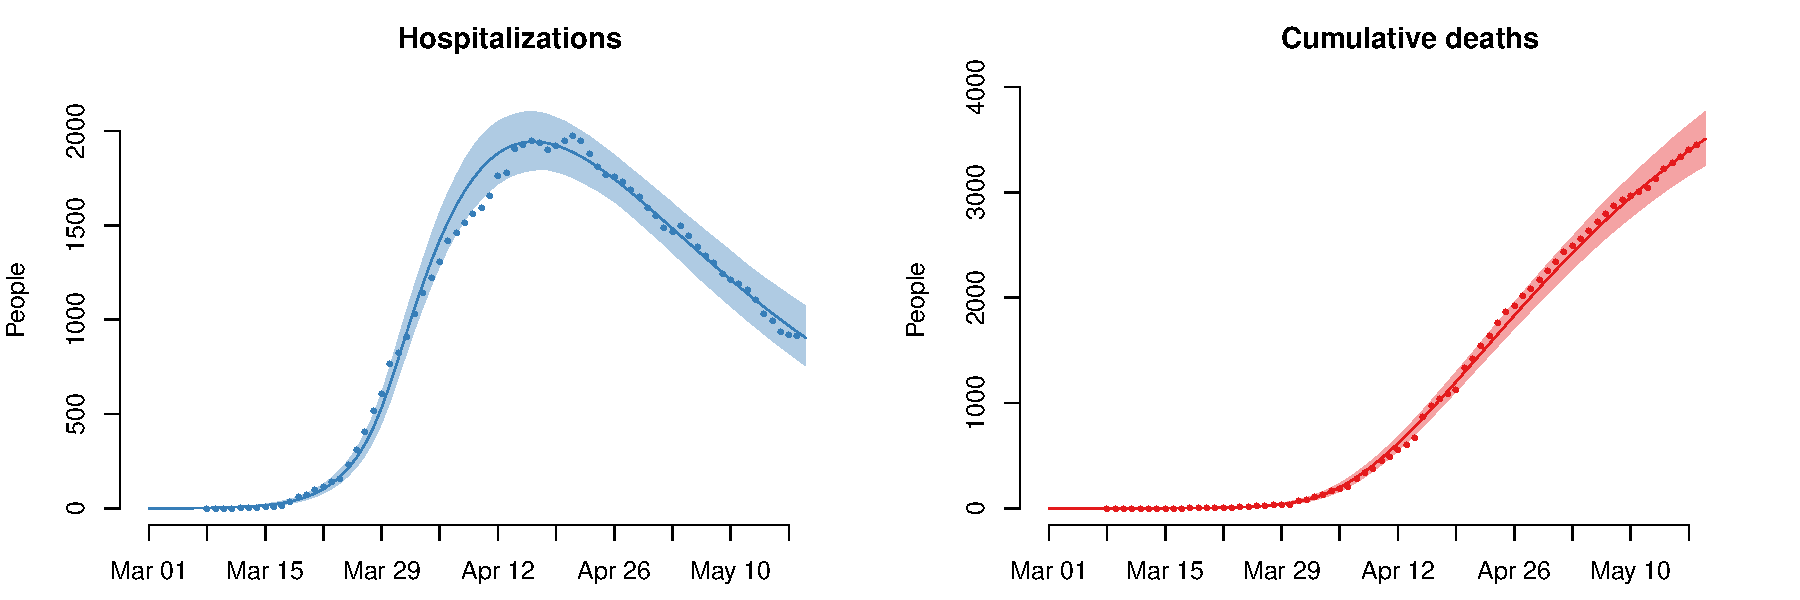
\includegraphics[width=.8\textwidth]{figures/calibration.pdf}
	\caption{Parameter calibration results under the low asymptomatic fraction scenario ($q_A = 0.36$).}
	\label{fig:fit}
\end{figure}



%%%%%%%% posterior distributions of parameters %%%%%%

%\begin{spacing}{1.25}
\begin{table}
	\centering
	\caption{Means and 95\% credible interval of marginal posterior distributions of model parameters under the low ($q_A = 0.36$), medium ($q_A = 0.5$), and high ($q_A = 0.7$) asymptomatic fraction scenarios.}
	\begin{tabular}{rrrrrrrrrr}
		\hline
		Parameter & \multicolumn{3}{c}{low asymptomatic} & \multicolumn{3}{c}{medium asymptomatic} & \multicolumn{3}{c}{high asymptomatic} \\
		{} & mean & CI-low & CI-high & mean & CI-low & CI-high & mean & CI-low & CI-high \\ 
		\hline
		$q_Is$ & 0.063 & 0.040 & 0.086 & 0.050 & 0.028 & 0.073 & 0.028 & 0.015 & 0.042 \\ 
		$\beta$ & 1.302 & 1.152 & 1.447 & 1.566 & 1.359 & 1.797 & 2.024 & 1.681 & 2.435 \\ 
		$\gamma_H$ & 0.115 & 0.099 & 0.131 & 0.113 & 0.095 & 0.131 & 0.115 & 0.095 & 0.134 \\ 
		$\gamma_U$ & 0.071 & 0.053 & 0.088 & 0.071 & 0.052 & 0.090 & 0.072 & 0.054 & 0.094 \\ 
		$k_A$ & 0.395 & 0.305 & 0.495 & 0.403 & 0.306 & 0.501 & 0.392 & 0.289 & 0.502 \\ 
		$k_Is$ & 0.697 & 0.603 & 0.796 & 0.698 & 0.606 & 0.795 & 0.707 & 0.599 & 0.798 \\ 
		$m_H$ & 0.209 & 0.186 & 0.231 & 0.209 & 0.183 & 0.232 & 0.208 & 0.185 & 0.232 \\ 
		$m_U$ & 0.307 & 0.247 & 0.375 & 0.309 & 0.239 & 0.379 & 0.308 & 0.248 & 0.385 \\ 
		$q_H$ & 0.572 & 0.520 & 0.617 & 0.573 & 0.519 & 0.620 & 0.574 & 0.524 & 0.622 \\ 
		$w\textsubscript{school}$ & 0.149 & 0.123 & 0.177 & 0.150 & 0.120 & 0.177 & 0.151 & 0.121 & 0.178 \\ 
		$w\textsubscript{lockdown}$ & 0.700 & 0.659 & 0.738 & 0.711 & 0.674 & 0.748 & 0.714 & 0.678 & 0.761 \\ 
		\hline
	\end{tabular}
	\label{tbl:posterior}
\end{table}
%\end{spacing}


%%%%%%%%% projections %%%%%%%%%%%%

\begin{figure} %[htb]
	\centering
	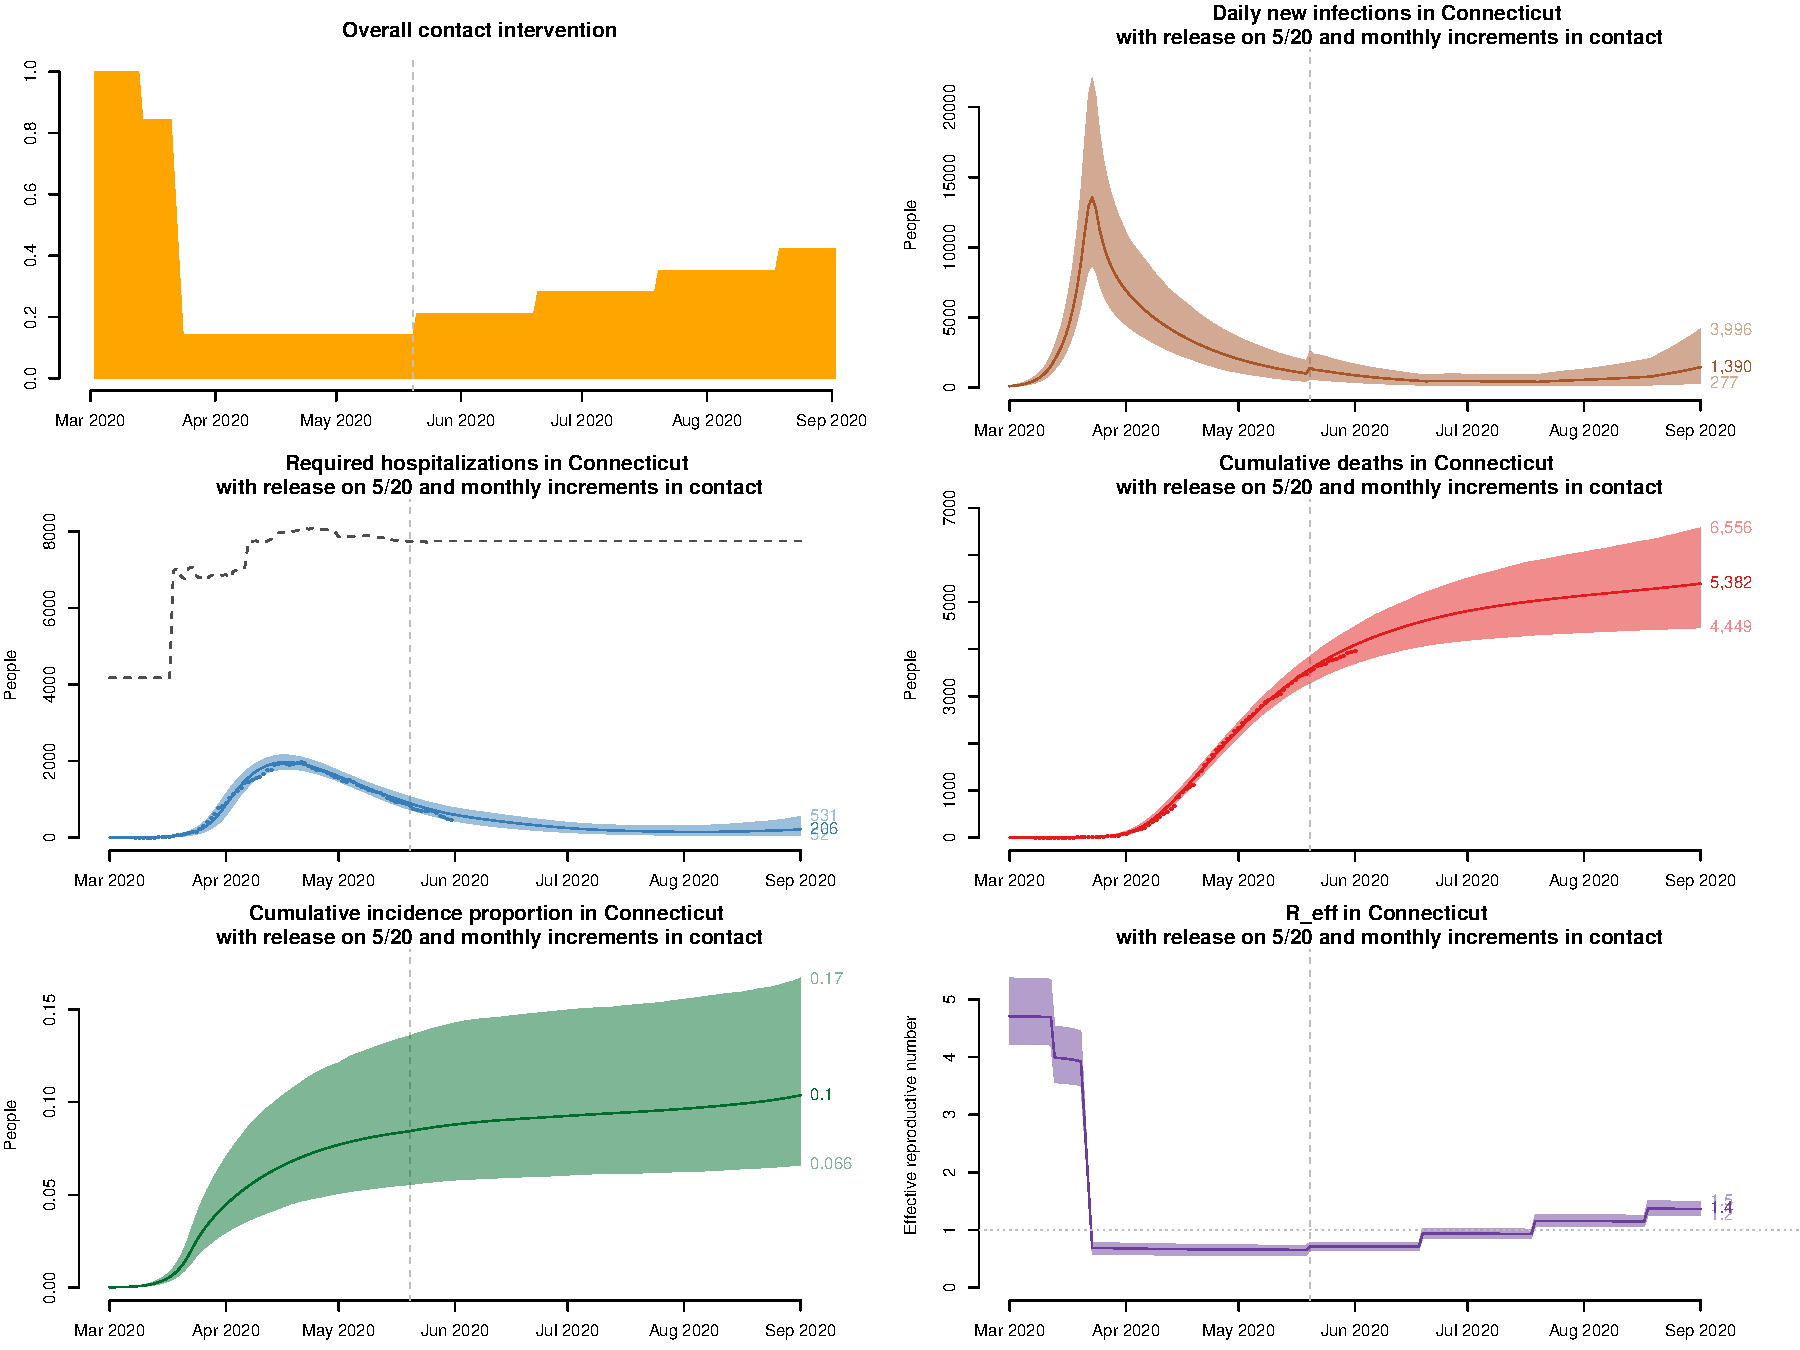
\includegraphics[width=.9\textwidth]{figures/slow_low_full.pdf}
	\caption{Projections under a ``slow'' reopening scenario and Scenario 1, low asymptomatic proportion. 10\% of suppressed contact is released every 30 days, starting on May 20, 2020, with 95\% uncertainty intervals. The dashed line above hospitalization projections is an estimate of the hospital bed capacity in Connecticut \citep{CHAwebsite}. }
	\label{fig:slow_low}
\end{figure}

\begin{figure} %[htb]
	\centering
	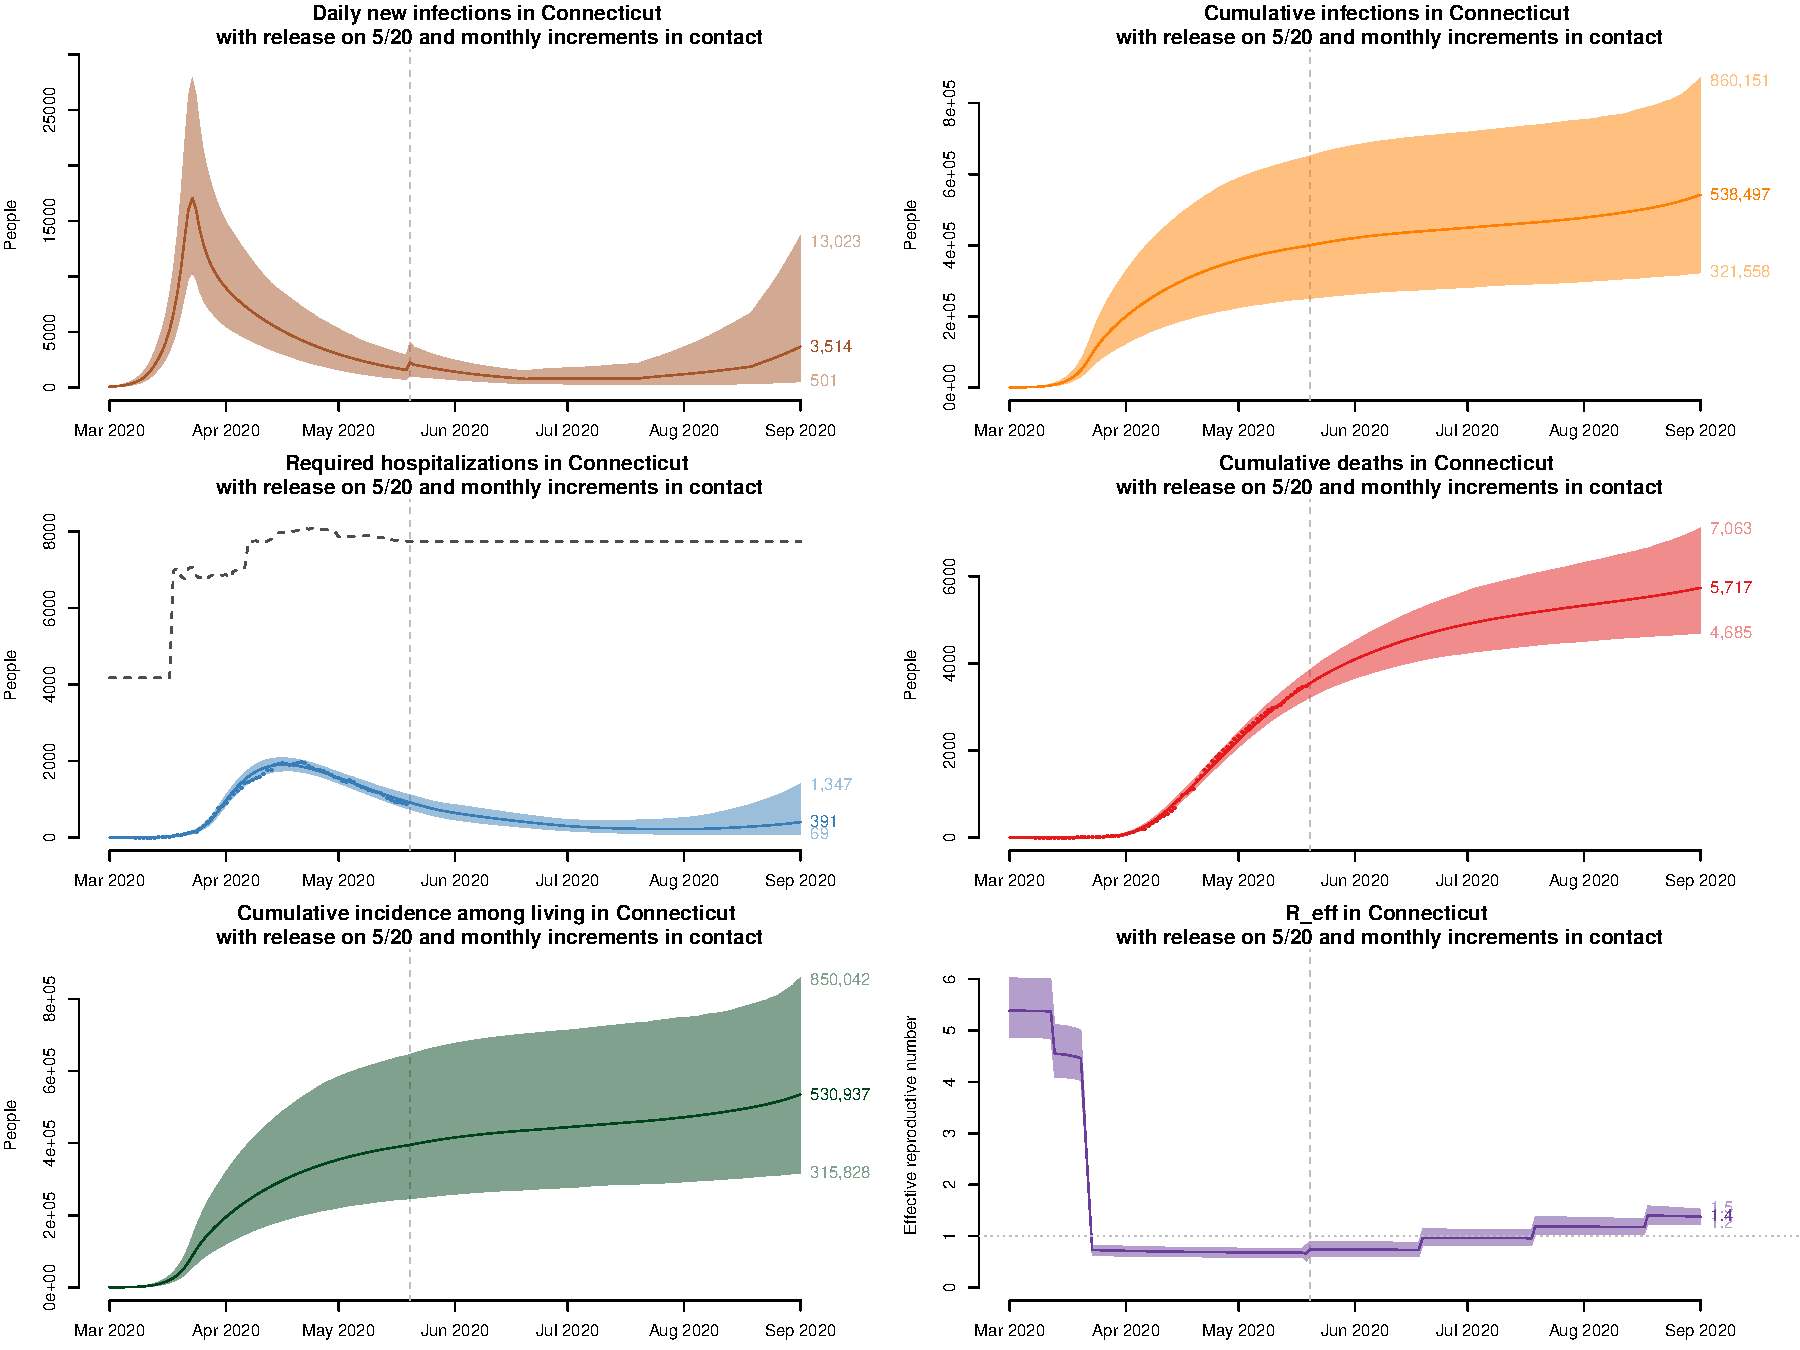
\includegraphics[width=.9\textwidth]{figures/slow_medium_full.pdf}
	\caption{Projections under a ``slow'' reopening scenario and Scenario 2, medium asymptomatic proportion. 10\% of suppressed contact is released every 30 days, starting on May 20, 2020, with 95\% uncertainty intervals. The dashed line above hospitalization projections is an estimate of the hospital bed capacity in Connecticut \citep{CHAwebsite}. }
	\label{fig:slow_medium}
\end{figure}

\begin{figure} %[htb]
	\centering
	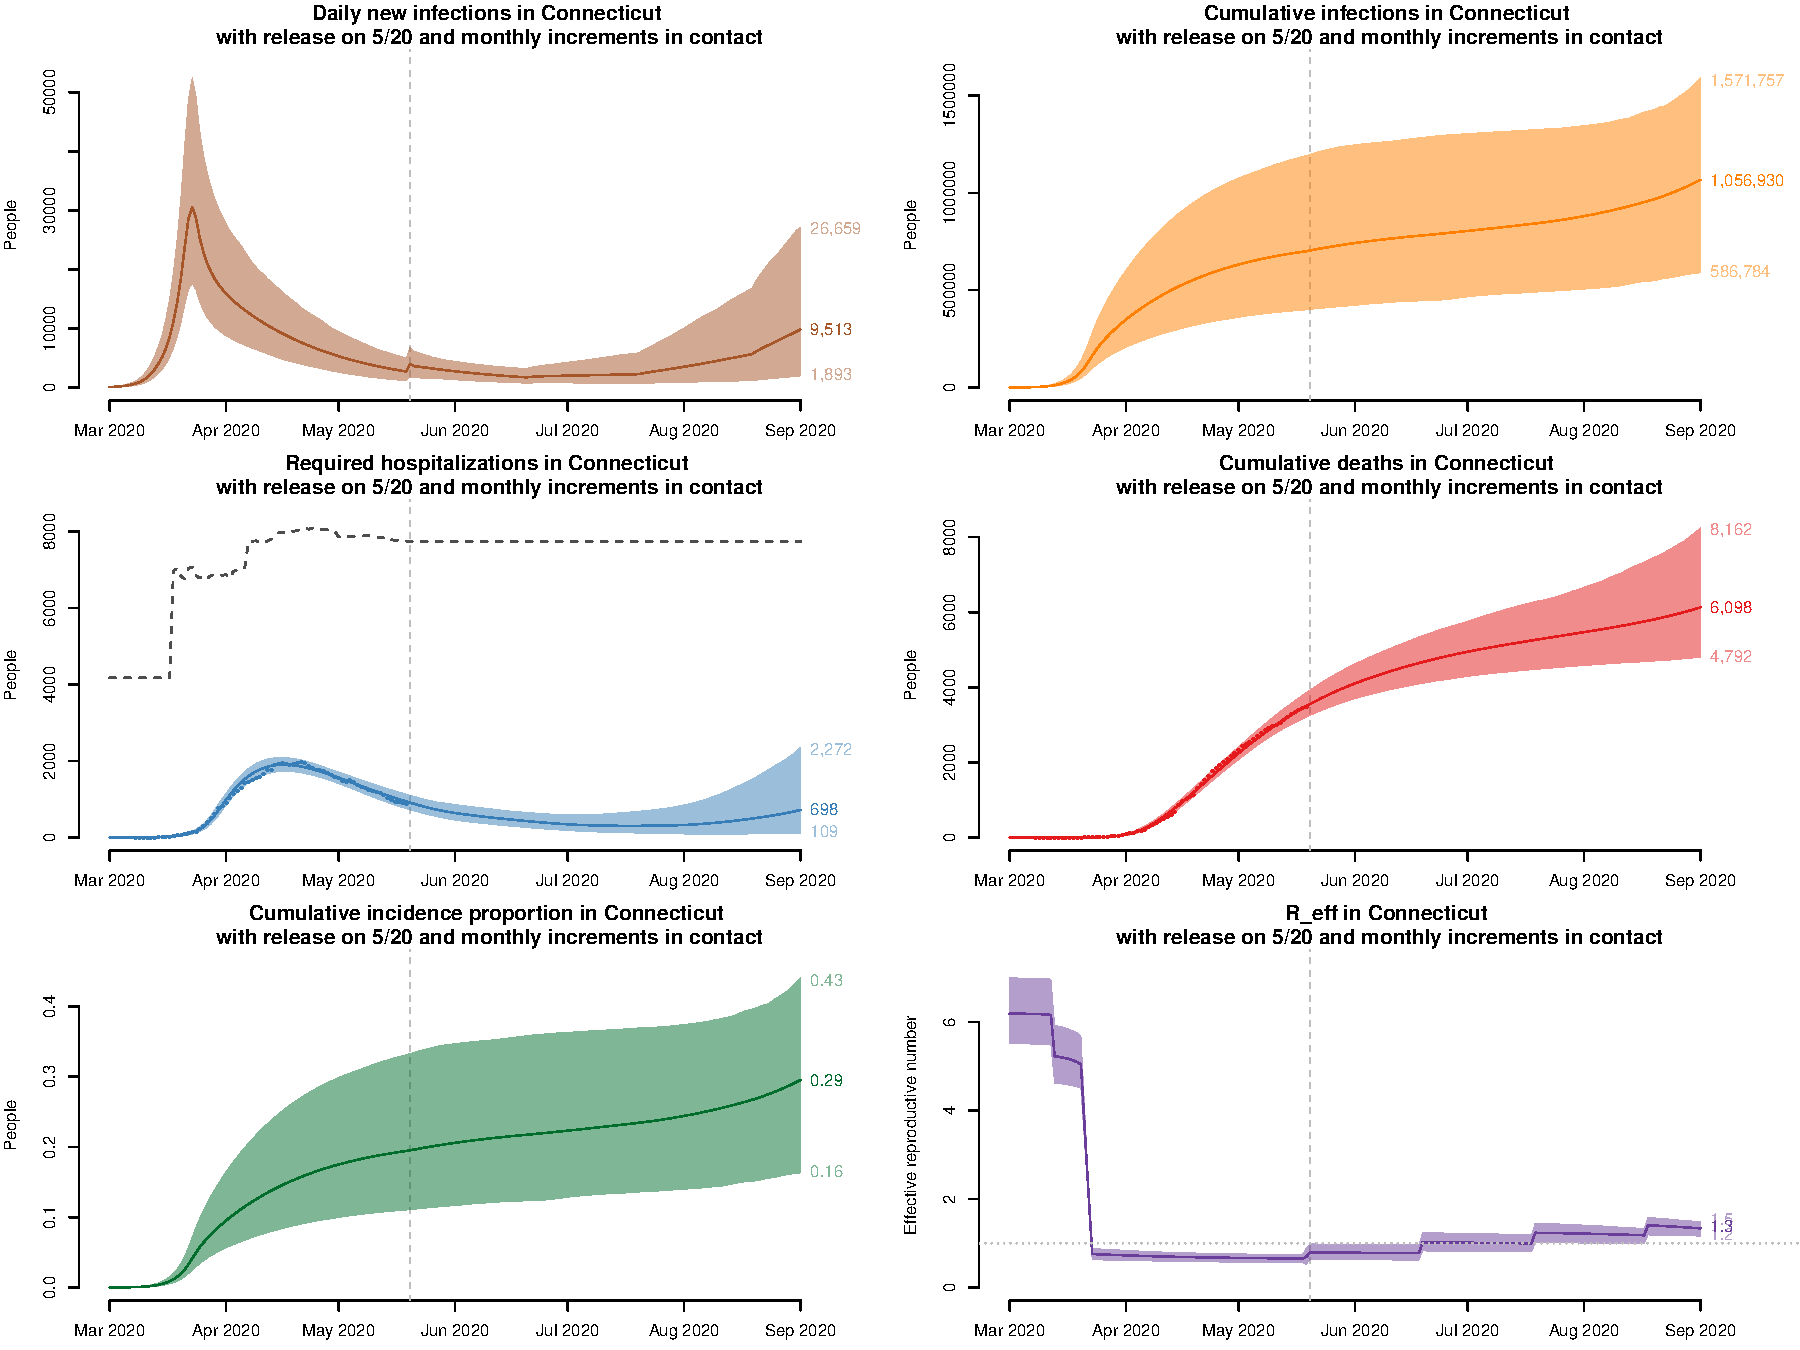
\includegraphics[width=.9\textwidth]{figures/slow_high_full.pdf}
	\caption{Projections under a ``slow'' reopening scenario and Scenario 3, high asymptomatic proportion. 10\% of suppressed contact is released every 30 days, starting on May 20, 2020, with 95\% uncertainty intervals. The dashed line above hospitalization projections is an estimate of the hospital bed capacity in Connecticut \citep{CHAwebsite}. }
	\label{fig:slow_high}
\end{figure}


\begin{figure} %[htb]
	\centering
	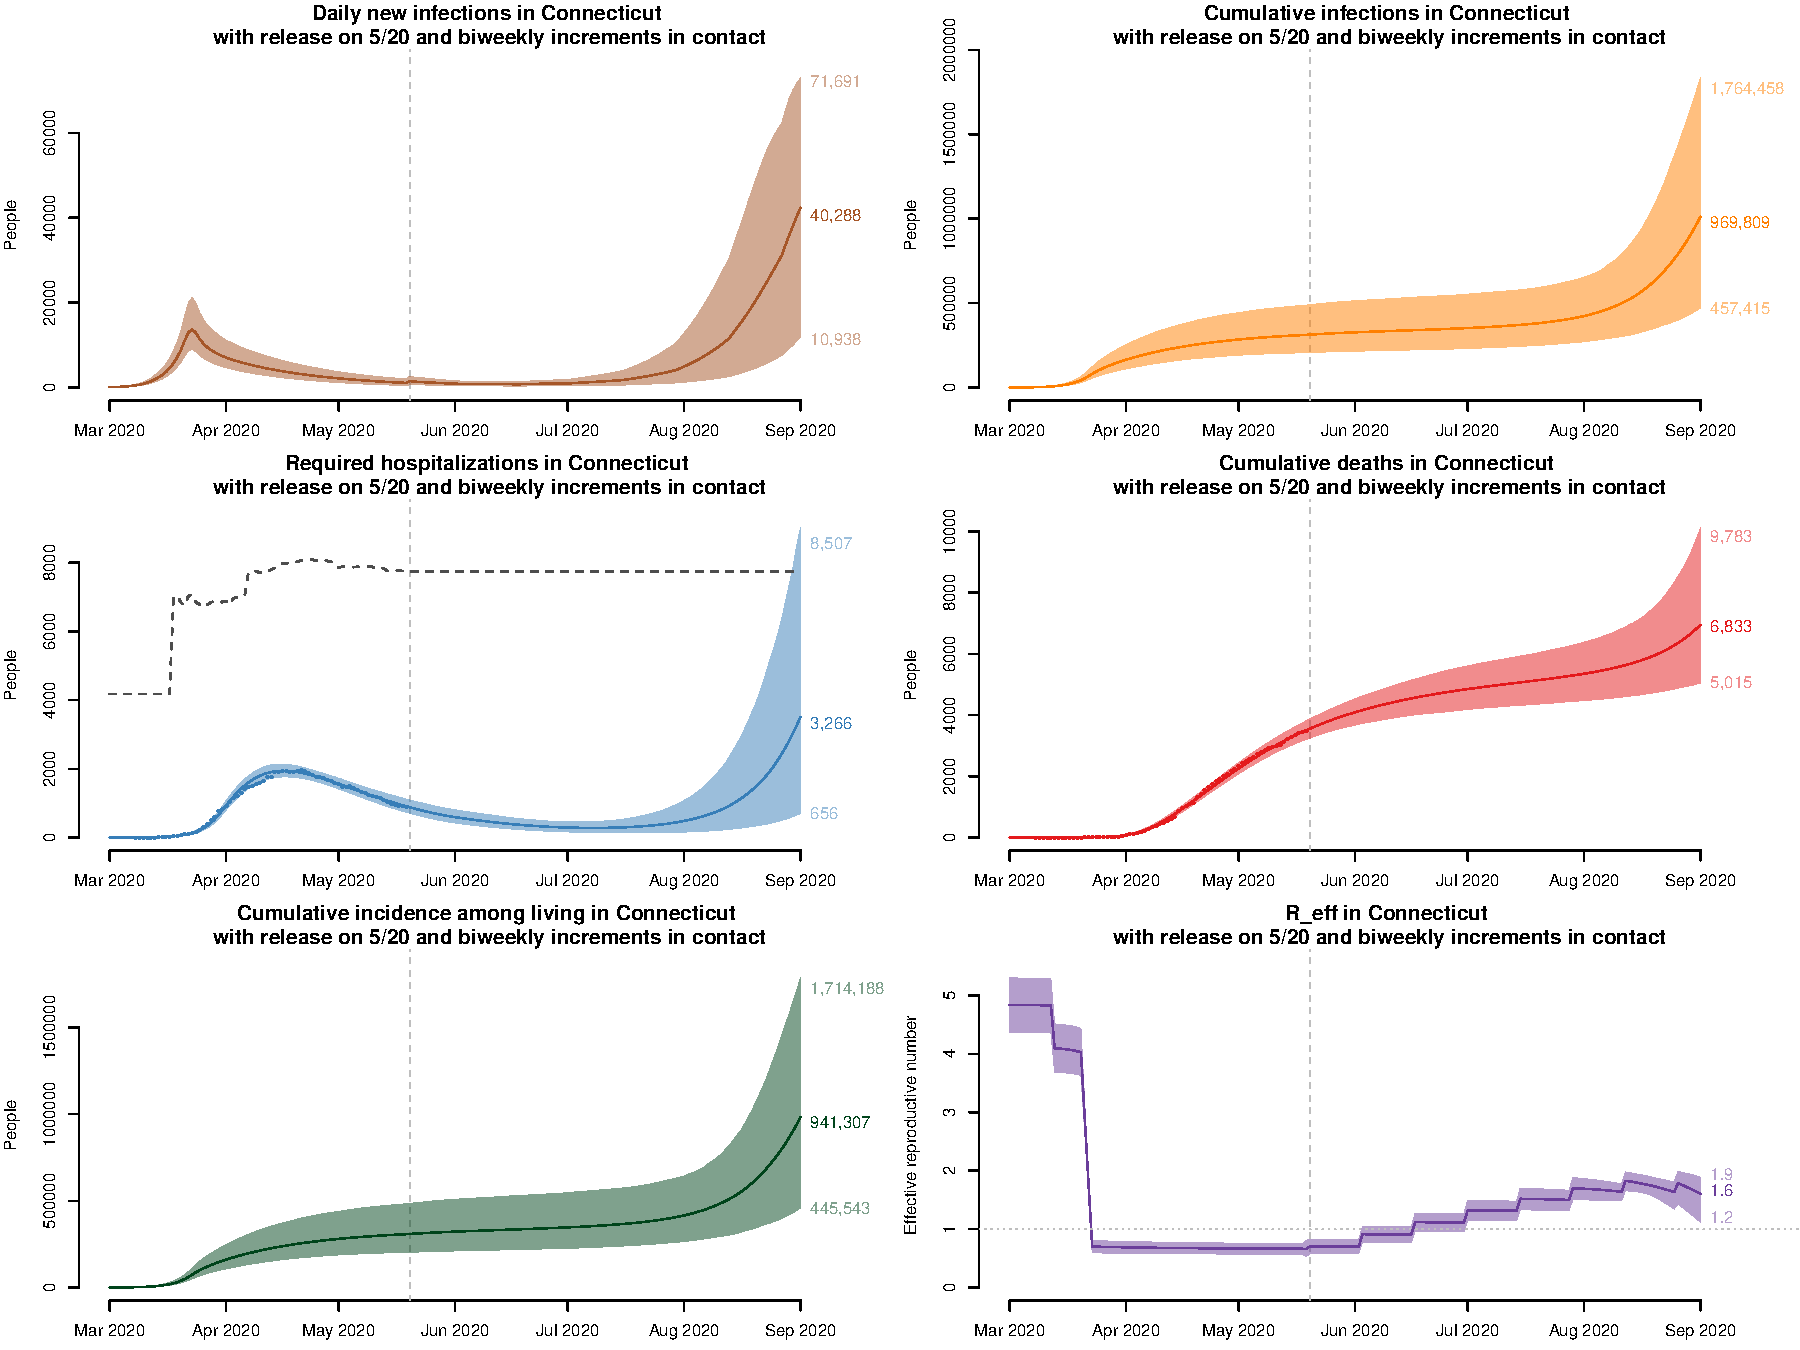
\includegraphics[width=.9\textwidth]{figures/fast_low_full.pdf}
	\caption{Projections under a ``fast'' reopening scenario and Scenario 1, low asymptomatic proportion. 10\% of suppressed contact is released every 30 days, starting on May 20, 2020, with 95\% uncertainty intervals. The dashed line above hospitalization projections is an estimate of the hospital bed capacity in Connecticut \citep{CHAwebsite}. }
	\label{fig:fast_low}
\end{figure}

\begin{figure} %[htb]
	\centering
	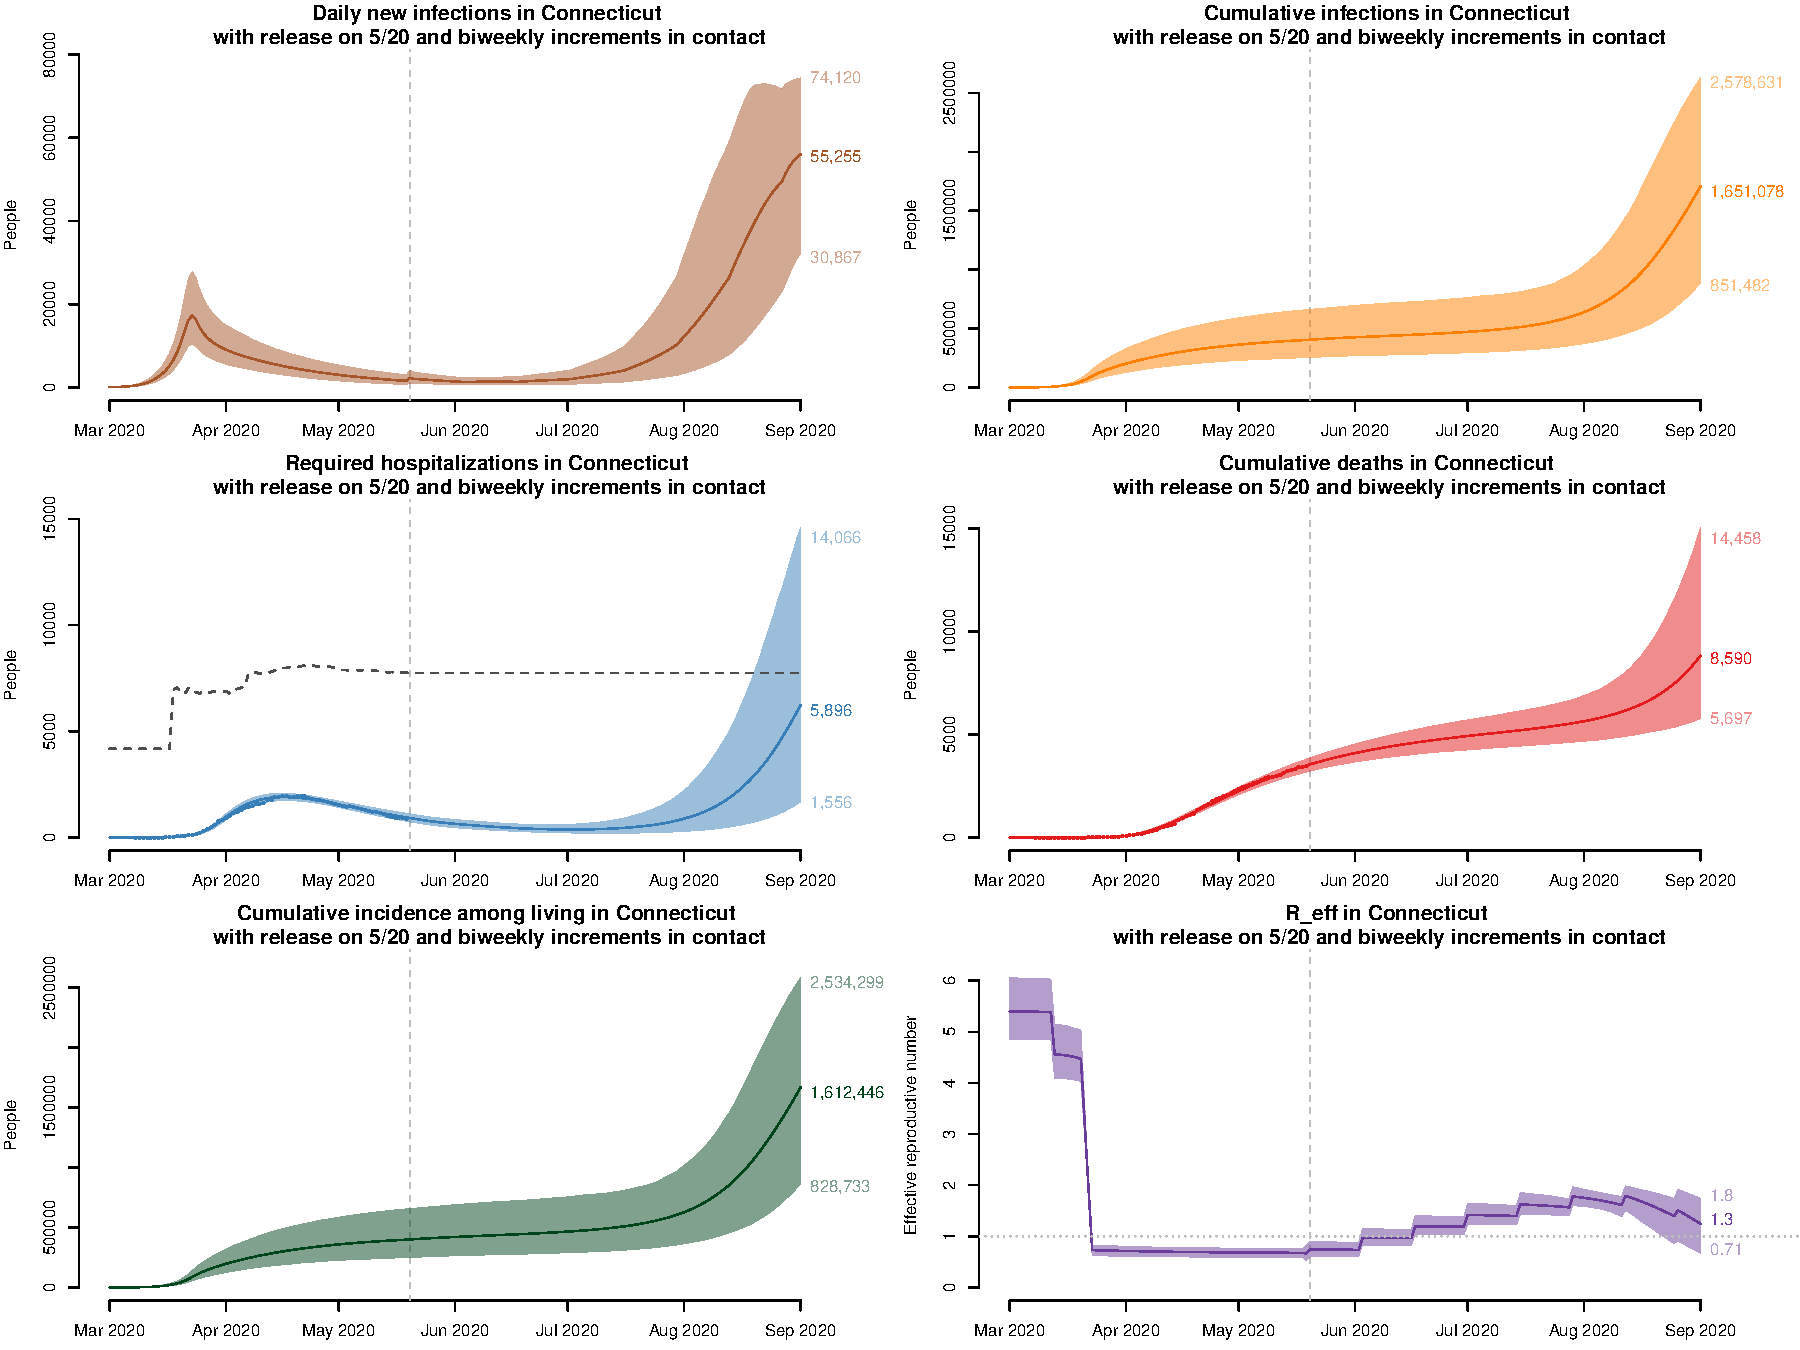
\includegraphics[width=.9\textwidth]{figures/fast_medium_full.pdf}
	\caption{Projections under a ``fast'' reopening scenario and Scenario 2, medium asymptomatic proportion. 10\% of suppressed contact is released every 30 days, starting on May 20, 2020, with 95\% uncertainty intervals. The dashed line above hospitalization projections is an estimate of the hospital bed capacity in Connecticut \citep{CHAwebsite}. }
	\label{fig:fast_medium}
\end{figure}

\begin{figure} %[htb]
	\centering
	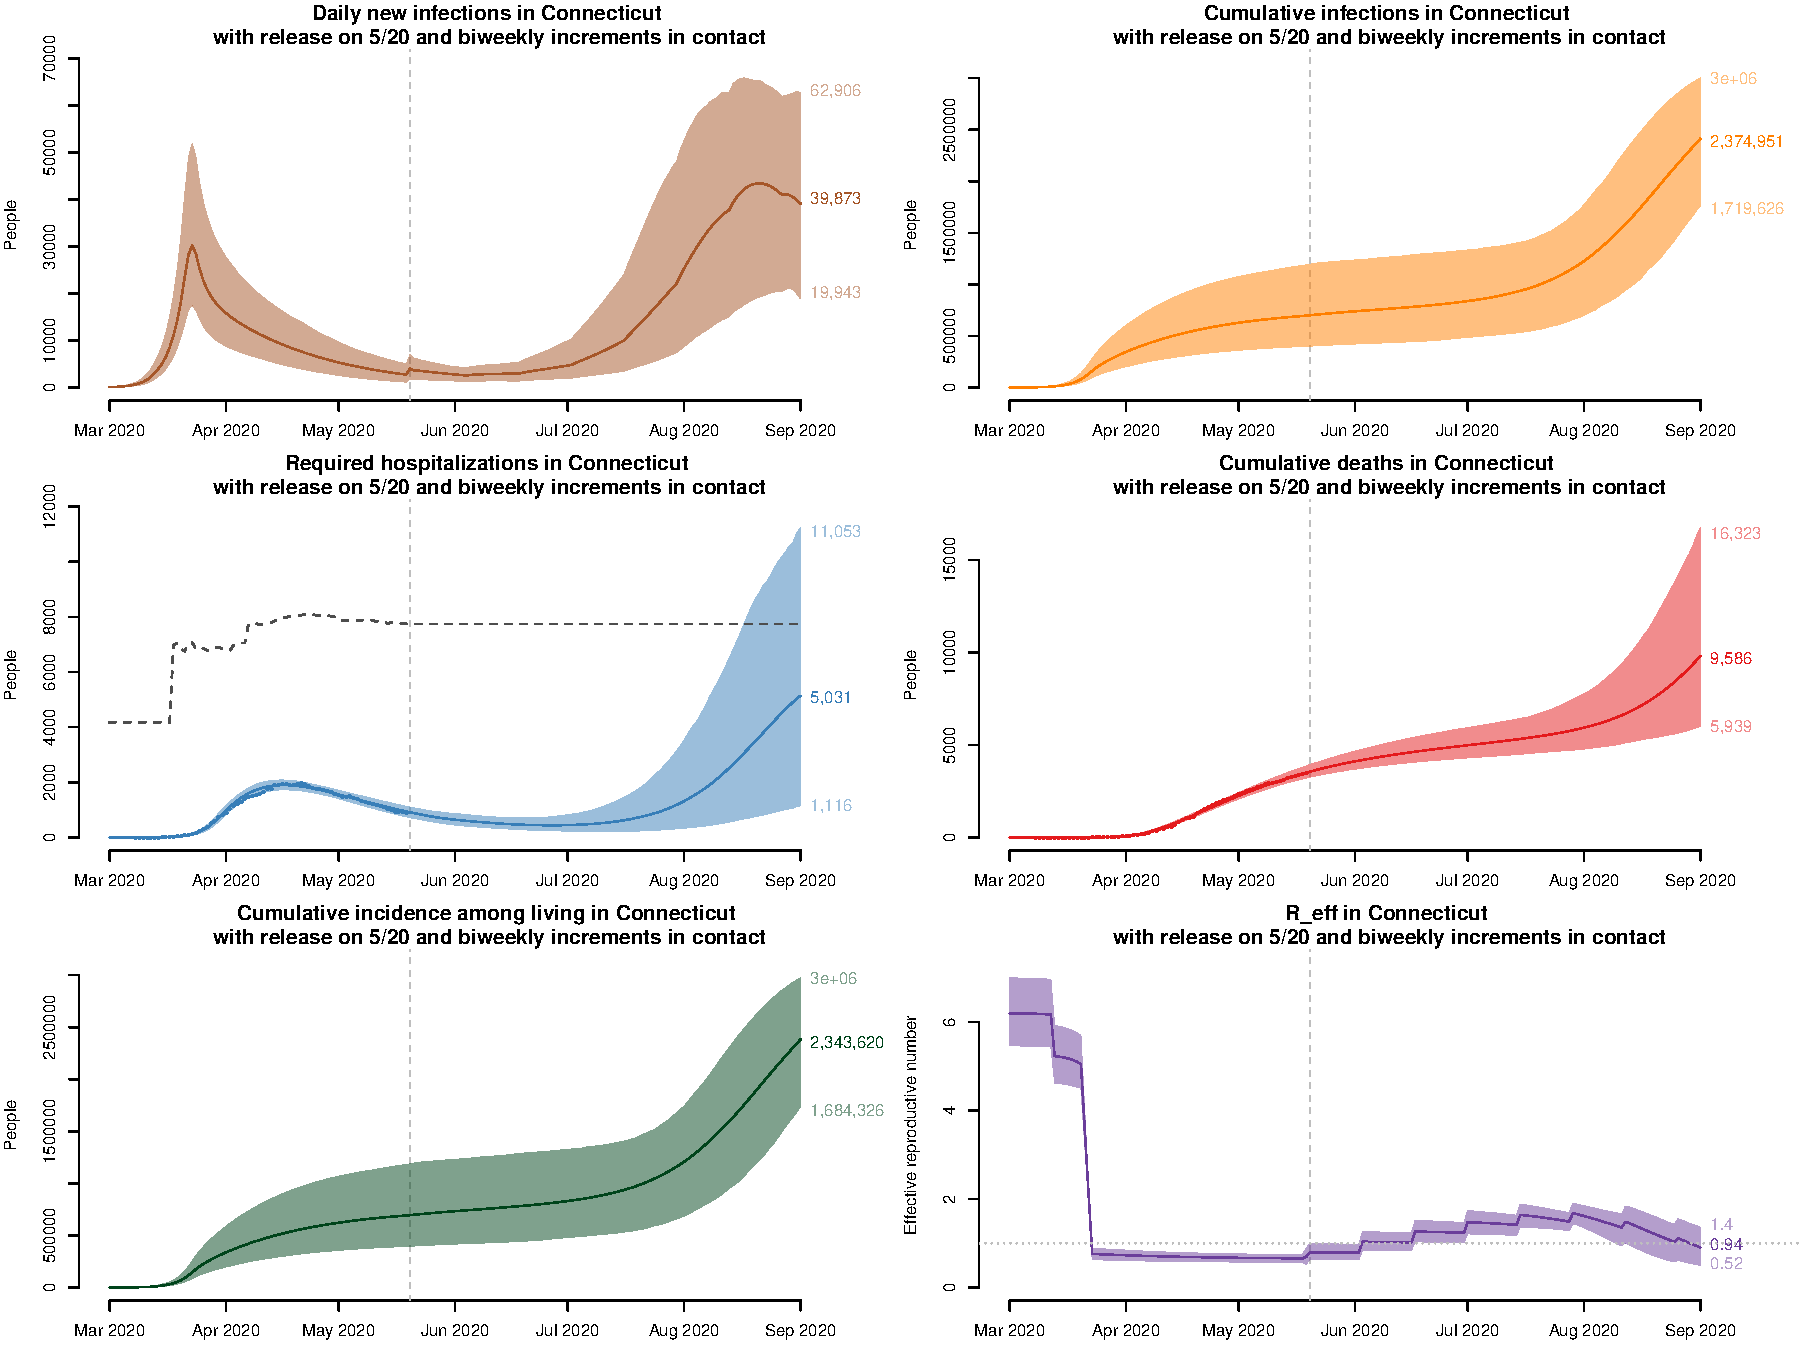
\includegraphics[width=.9\textwidth]{figures/fast_high_full.pdf}
	\caption{Projections under a ``fast'' reopening scenario and Scenario 3, high asymptomatic proportion. 10\% of suppressed contact is released every 30 days, starting on May 20, 2020, with 95\% uncertainty intervals. The dashed line above hospitalization projections is an estimate of the hospital bed capacity in Connecticut \citep{CHAwebsite}. }
	\label{fig:fast_high}
\end{figure}








%%%%%%%%%%%%%%%%%%

\section{Discussion}

%\comments{Contextualize the model structure by comparing it to others. This can be short.} 

%\comments{When comparing IHME, probably mention we use all beds as capacity instead of available beds. IHME capacity is about 1/4 ours.}

In this report, we have described technical details of a model of SARS-CoV-2 transmission and COVID-19 disease progression developed to support public health decision-making in Connecticut.  The model is calibrated to the observed dynamics of hospitalizations and cumulative deaths in Connecticut; its projections reproduce these dynamics accurately.  Many COVID-19 models have been developed and analyzed by the CDC in the attempt to perform ensemble forecasting of the epidemic development in the US \citep{cdc2020covid19forecasts}. Most of these models offer state-level projections. The CDC publishes updates of consolidated summary of cumulative death projections in the next four weeks from these models for each state. Local projections from national-level models may offer useful insights, but they inevitably make simplifying or uniform assumptions, which may hold in some locations, but not others. 


There is substantial uncertainty about epidemiologic parameters that govern aspects of COVID-19 dynamics and have a direct impact on the quality of projections. When local context is not directly taken into account, the effects of parametric uncertainty is exacerbated.  State and county-level models are needed to support local decision-making.  The model described here captures distinct important features of COVID-19 dynamics and the relationship between model features and data reporting in Connecticut.  By calibrating model parameters to local data, including changes in hospitalization capacity, and the exact timing of intervention events, we can reduce uncertainty in projections. However, the calibrated posterior distribution of model parameters is not necessarily generalizable to other settings: model projections are tightly linked to the Connecticut reopening plans. 

In addition to providing predictions for policymakers, model projections may be useful for prospectively planning epidemiologic studies that can inform the state's response.  In particular, planning of seroprevalence surveys requires estimates of the proportion of population who have been exposed to the virus in the past or are in an active stage of infection. Due to limited testing availability and potentially high proportion of asymptomatic individuals, official case counts offer a poor approximation to the true cumulative incidence. Seroprevalence surveys, if properly conducted, can provide an important piece of information that would permit more precise estimates of the fraction of asymptomatic infections. 

Prior knowledge and assumptions about plausible ranges of parameter values combined with local data allows us to substantially reduce parametric uncertainty and produce narrow projection intervals. However, several important considerations limit our ability to make reliable long-term projections. First it is difficult to make predictions about the extent of contact rate increases following lockdown release steps, such as allowing only certain types of businesses to reopen. Second, the effectiveness of widespread testing and contact tracing on timely isolation of infectious individuals, and its subsequent impact on the force of infection is unknown. This effect is a complex function of viral shedding characteristics among symptomatic, presymptomatic and asymptomatic individuals, along with the implementation features of testing and isolation. Third, there may be unequal depletion of susceptibles depending on their severity risk profile. If a higher fraction of high-risk individuals have already experienced infection compared to low-risk individuals, then we may be over-estimating future number of deaths. Forth, we assume that all epidemiologic parameters are constant over time and are not subject to seasonal forcing. It is hypothesized that temperature may play a role in transmission dynamics beyond its impact on contact patterns \citep{kissler2020projecting}, in which case we would expect lower transmission intensity in summer all other things being equal.

In an evolving public health crisis, it is important to keep projections up to date. As more information about the extent of asymptomatic transmission, general epidemiologic characteristics of COVID-19, and data on observable model features in Connecticut becomes available, we will update the projections presented in this paper.




%%%%%%%%%%%%%%%%%%%%%%%%5

%\noindent \textbf{Acknowledgements}:
% We are grateful to [...]
% Eben Kenah
% Ira Longini
% Albert Ko
% Sten Vermund
% A. David Paltiel
% Peter M. Aronow,
% Xiaoxuan Cai,
% Fredrik S\"avje
% Daniel Weinberger
% Virginia E. Pitzer
% Who else?
%for helpful comments.



%%%%%%%%%%%%%%%%%%%%%%%%%%%%%%%%%%

\bibliographystyle{unsrtnat}

\bibliography{covid19}

\end{document}
